% ============================================================
% Pinning the Wage to Scarcity and Technology
% Task assignment, recursive machine production, and non-produced inputs.
% Numerical checks: check_interior.py in the source bundle.

% ============================================================
% Style: orthodox macro working paper (12pt, onehalf spacing, plain theorem
% style with italic statements, numbered equations, CM fonts).
\documentclass[12pt]{article}
\usepackage[T1]{fontenc}
\usepackage{lmodern}
\usepackage[utf8]{inputenc}
\usepackage[a4paper, margin=2.5cm]{geometry}
\usepackage{setspace}
\onehalfspacing
\clubpenalty=10000
\widowpenalty=10000
\usepackage{amsmath, amssymb, amsthm}
\usepackage{bm}
\usepackage{graphicx}
\usepackage{booktabs}
\usepackage[labelfont=bf, labelsep=period, font={footnotesize,stretch=1}, justification=justified]{caption}
\usepackage{microtype}
\usepackage{titlesec}
\usepackage[hidelinks]{hyperref}

\theoremstyle{plain}
\newtheorem{proposition}{Proposition}
\newtheorem{lemma}[proposition]{Lemma}
\newtheorem*{corollary}{Corollary}

% hanging-indent entry for the hand-formatted reference list
\newcommand{\refentry}[1]{\par\hangindent=1.5em\hangafter=1\noindent #1}

\title{\bfseries Pinning the Wage to Scarcity and Technology\thanks{Views are the
  authors' own and do not represent those of KTH, SEB, or the Stockholm School of
  Economics. Written in collaboration with Claude (Anthropic); see the AI-use note
  at the end.
  }\\[7pt]
  \large\mdseries Replacement, exit, and the rents of non-produced inputs in a task economy}

\author{
  Johan B\r{a}ge\thanks{Stockholm School of Economics.
    Email: \texttt{Johan.Bage@hhs.se}.
  }
  \and
  Stella Wilson\thanks{KTH Royal Institute of Technology and Skandinaviska
    Enskilda Banken (SEB). Email: \texttt{thmwi@kth.se}.}
}

\begin{document}
\maketitle

\begin{abstract}
\noindent We endogenize labor's replacement cost and workers' outside option in a task model with recursive machine production, linking both to rents on non-produced inputs. As machine production sheds labor, rents account for more of replacement cost, while rising rents reduce the outside option in goods units. At an interior task margin, we derive category prices and bounds on wage purchasing power from human productivity and direct requirements for non-produced inputs. The associated rent bill places a ceiling on purchasing power that falls with the wage--rent ratio. U.S. wage measures deflated by durables and shelter prices diverged by a factor of 4.8 over 1964--2024. Taxing pure rents to fund uniform transfers preserves fixed-factor supply and introduces no benefit withdrawal upon employment. Full capture of measured U.S. site rents could fund about one-third of a per-person subsistence bundle in 2025.
\end{abstract}

\section{Introduction}\label{sec:intro}

Suppose a firm can perform a task with a worker or with a machine. For the tasks where the firm is indifferent, the worker's wage is tied to the cost of the machine substitute. That mechanism is established and used by the factor-price condition at the task margin in Acemoglu and Restrepo (2018), with the same threshold logic in Zeira (1998) and, for tasks that move abroad rather than to machines, in Grossman and Rossi-Hansberg (2008). This paper examines that mechanism with two questions around that margin.

\textbf{What prices the substitute?} A machine is itself produced --- from other machines, labor, energy, sites, minerals, permissions. Its rental is an equilibrium object. Tracing the machine rental through its input costs eventually leads to non-produced inputs: resources whose supply is not generated by the production process. Land and mineral deposits are examples. A grid connection or fabrication bottleneck can hold the same position over shorter horizons, while its capacity is fixed. While machine production still employs labor, part of the machine's cost will be the wage itself, and thus the substitute will remain relatively expensive. As machine production sheds labor, that cost component is reduced, and such ``terminal'' rents account for an increasing share of the replacement price.

\textbf{What prices the alternative to working at all?} A worker sells an hour when the wage beats the best alternative use of that hour. Life outside the market wage still requires somewhere to live, food, energy, warmth, and usually access to a household. The value of exit is therefore also a price --- and it depends on the same scarce inputs that anchor the machine's cost. When machine-made goods cheapen while housing and energy do not, the outside option falls in the consumption units relevant to participation toward a ``participation floor,'' and its lower bound, the ``dependency floor''.

This paper endogenizes the two prices that bound the labor margin. On the demand side,
\[
\textit{labor demand} \to \textit{replacement cost} \to \textit{terminal rents};
\]
on the supply side,
\[
\textit{labor supply} \to \textit{outside option} \to \textit{terminal rents}.
\]
Replacement cost is the firm's opportunity cost of employing labor; the outside option is the worker's opportunity cost of supplying it. Both are formed partly in the market for non-produced inputs. Technological change therefore moves the two sides together: it changes relative capability at final tasks (``task automation''), the labor embodied in machine production (``recursive automation''), and the relative price of the scarce inputs at which both chains terminate.

At an interior task margin, the wage relative to rent links automation to purchasing power. At a given marginal task and machine recipe, a fall in relative human productivity lowers the wage relative to terminal rent; removing labor from the machine recipe lowers it further. Category prices combine task costs with direct requirements for non-produced inputs. A category must cover the associated rent bill, placing an upper bound on the quantity an hour's wage can buy. A feasible human method supplies the complementary lower bound through its labor cost and rent bill. The two bounds describe purchasing power as humans and machines divide the tasks of production. In the model with one non-produced input, if the wage--rent ratio tends to zero, wage purchasing power tends to zero for categories whose direct requirement remains bounded away from zero. Categories with no direct requirement and bounded human production hours retain a positive lower bound set by human productivity.

Combining the task margin of Acemoglu and Restrepo with the input--output price logic of Leontief (1936) and Sraffa (1960), and pricing the outside option in the same relative price, yields the real-wage fork. The resulting distinction between wage and ownership income motivates the policy pair associated with George (1879): a tax on pure rents funding a uniform transfer.

The next section locates the contribution in the wage-determination
literature. The main text then develops the task and outside-option closures,
derives the interior purchasing-power and income results, and turns to history,
measurement, stabilizers, and AI. The appendices provide the general
environment, transition results, and extensions.

\section{How existing literature characterizes the wage}\label{sec:accounts}

Accounts of the aggregate wage differ less in their mechanisms than in where they stop. Each family below determines the wage relative to a quantity that labor itself helps produce, or leaves it inside an interval whose endpoints it takes as given, or determines its growth rate while not fixing its level. We do not present the model of Sections~\ref{sec:model}--\ref{sec:floor} as an alternative to these accounts. Instead, we focus on the objects they take as given.

\subsection{Marginal product}\label{sec:marginal-product}

The textbook answer sets the wage equal to the marginal product of labor. As a statement about competitive equilibrium it is correct, and this paper's Proposition~\ref{prop:margin} is an instance of it: $w = c\cdot \gamma (x^*)$  is the marginal product, evaluated at the margin the machine alternative sets. What the identity does not supply is a level: the marginal product is a function of the capital stock and the technology, two variables constantly changing. Applied work often proceeds under Cobb--Douglas, which imposes fixed factor shares and requires an aggregate capital measure. Both assumptions become fragile when factor shares and capital prices are themselves moving rapidly (Sraffa 1960; Samuelson 1966). In growth theory the wage's growth rate is pinned along a balanced path, but Uzawa (1961) shows the balanced path requires technical change to be labor-augmenting in form --- and the form of technical change is precisely what is at issue under automation.

\subsection{Search, matching, and bargaining}\label{sec:search}

The search-and-matching framework (Diamond 1982; Mortensen and Pissarides 1994; Pissarides 2000) places the wage between the worker's outside option and the value of the match, dividing the surplus by a bargaining parameter. The framework is explicit that the level is not determined within it: two endpoints and a split, and it supplies none of the three.

Shimer (2005) showed that the calibrated model generates almost none of the observed volatility --- in U.S. data the vacancy--unemployment ratio is roughly twenty times as volatile as labor productivity, while the model makes them comparable. Hagedorn and Manovskii (2008) resolve the puzzle by setting the value of non-market activity close to productivity, so that the surplus workers and firms split is small; Hall (2005) resolves it with rigid wages; and Ljungqvist and Sargent (2017) show that these and the other proposed resolutions operate through one channel, the \emph{fundamental surplus} --- ``an upper bound on the fraction of a job's output that the invisible hand can allocate to vacancy creation'' --- which every successful calibration makes small, and whose leading deduction from productivity is the value of non-work. The central calibration debate of modern macro-labor is, in other words, a debate about the level of an object the framework treats as a parameter.

Our contribution is to endogenize both endpoints --- the firm's machine alternative and the worker's outside option --- and to show that both depend partly on the same scarcity market.

\subsection{Task and assignment models}\label{sec:tasks}

The task framework (Zeira 1998; Acemoglu and Autor 2011; Acemoglu and Restrepo 2018, 2022) determines the wage at the threshold task and is the direct ancestor of what follows. Its equilibrating force is the creation of new labor tasks: displacement met by reinstatement (Acemoglu and Restrepo 2018; Autor 2015). In each version the machine rental and the outside option enter as parameters; the wage is passed through the threshold rather than determined at it. This paper endogenizes both parameters and abstracts from the creation of new labor tasks, a modeling choice motivated by our reading of history and recent U.S. measures. Acemoglu and Restrepo (2026) add institutional wage wedges and show that automation is directed at the tasks where wedges are largest;  Cross-border trade is treated similarly: a tradable task stays domestically only while the wage beats both the machine rental and the foreign wage, so the foreign wage is a second machine rental with a different cost composition. Offshoring is still a temporary condition: once the machine undercuts the foreign worker, the task shifts onward to machines wherever they sit.

\subsection{Institutional accounts}\label{sec:institutions}

Efficiency wages (Shapiro and Stiglitz 1984), monopsony (Manning 2003), and firm-level rent sharing (Card, Cardoso, Heining, and Kline 2018) explain why individual wages depart from a common base and why the dispersion moves. In the notation below they are accounts of a multiplicative wedge on particular tasks. The model takes them as given at that layer and focuses instead on the common base.

\subsection{The classical accounts}\label{sec:classical}

The wage was pinned to land and to the cost of subsistence before it was pinned to anything else. Ricardo (1817) priced land at the margin and the wage at its natural price, Malthus (1798) supplying the mechanism; the machinery chapter added in 1821 concedes that machinery can injure the laboring class. Marx priced labor power at its cost of reproduction and read enclosure --- the legal extinction of common access to land --- as the manufacture of a labor supply. Lewis (1954) pinned the modern-sector wage to what the traditional sector affords --- the closest antecedent to our participation mechanism, differing in that his traditional sector is exhausted by absorption rather than priced away by rent. Polanyi (1944) recorded the institutional half of the same event. George (1879) drew the fiscal consequence derived below inside the model. These accounts were not refuted. The premise they shared --- that the human advantage over tools varied little from task to task --- stopped holding, and the conclusions lapsed with it. This is the classical configuration of the schedule.

\subsection{Automation and the wage}\label{sec:automation}

Korinek and Stiglitz (2019) pose the below-subsistence scenario this model resolves through exit; Korinek and Suh (2024) is the closest formal predecessor on wage collapse under transformative AI, differing in where the collapse ends --- here at non-produced factors rather than accumulated capital --- and in the treatment of the outside option. Susskind (2017) and Sachs and Kotlikoff (2012) reach technological immiseration through other channels; Moll, Rachel, and Restrepo (2022) route automation's gains to wealth-holders, where this model identifies the fixed-supply input to which the residual income accrues. Aghion, Jones, and Jones (2019) supply the strongest stabilizer --- expenditure concentrating on whatever remains human-required --- granted a theorem in Appendix~\ref{app:human}. Caselli and Manning (2019) prove that real wages cannot fall in terms of goods produced entirely from reproducible inputs; Section~\ref{sec:limit} gives a human-production lower bound for categories without direct requirements for non-produced inputs and shows how persistent requirements constrain other categories. Hémous and Olsen (2022) endogenize automation's direction.

\subsection{Other empirical measures}\label{sec:data}

Three empirical objects meet the model below. Factor shares: the labor share's decline is documented and global (Karabarbounis and Neiman 2014), and its capital-side counterpart resolves substantially into housing --- which is to say land (Rognlie 2015; Knoll, Schularick, and Steger 2017; Piketty and Zucman 2014). The long wage record: real wages measured against the cost of a subsistence basket --- welfare ratios in the sense of Allen (2001), extended for England by Clark (2005) --- are the same object this paper refers to as the participation floor, computed at the household level. Payroll incidence: the quasi-experimental literature (Gruber 1997; Kugler and Kugler 2009; Saez, Schoefer, and Seim 2019) provides evidence about labor-demand and participation elasticities. Schedule slope contributes to these elasticities, but incidence alone does not identify it when machine prices, output, and participation also respond.

\section{The model: task assignment and replacement cost}\label{sec:model}

\subsection{Tasks and the assignment margin}

\textbf{Tasks.} Producing one unit of the final good requires a continuum of tasks
$x \in [0,1]$, each in equal amount (Leontief aggregation over tasks): the good's
unit cost is the sum of its tasks' unit costs. One human-hour completes
$\gamma_L(x)$ units of task $x$; one machine-hour completes $\gamma_M(x)$.
Relative human productivity is
\begin{equation}\label{eq:gamma}
\gamma(x) = \gamma_L(x) / \gamma_M(x).
\end{equation}

A machine-hour rents for $c$. We begin by treating $c$ as given and then price it
from the machine sector's own production recipe below. Institutional wage wedges
--- union premia, licensing rents, efficiency wages --- are set aside until
Section~\ref{sec:stabilizers}.

\textbf{People and non-produced inputs.} $N$ identical workers each supply one hour or exit to an
outside option worth $s$ --- the value of the best life available without selling
labor. $s$ is a parameter here and is priced in Section~\ref{sec:floor}; it
presupposes access to the resources needed outside work. The baseline has one
non-produced input with a fixed stock. Land services provide a concrete example:
parcels differ in quality, and idle parcels have reservation rent zero.

Labor, at wage $w$, holds task $x$ when it is the cheaper input:
$w/\gamma_L(x) \le c/\gamma_M(x)$, i.e.
$w \le c\cdot\gamma(x)$. The right-hand side is labor's \emph{replacement value} at task $x$: the wage at which labor and the machine alternative cost the same there. Relabel tasks so $\gamma$ increases, and assume the
relabeled schedule is continuous and strictly increasing where labor is employed
(ties permit more than one cost-minimizing assignment). Some tasks cannot be performed by machines at any price:
$\gamma_M(x)=0$ there, so relative human productivity is unbounded.
Let $H$ denote the set of tasks closed to machines. The relabeling places
these tasks last, and Figure~\ref{fig:schedule} represents them as a wall at
the right edge of the schedule. Where labor holds at least one
machine-contestable task, $x^*$ denotes the marginal such task and the usual
indifference condition applies. If labor holds only tasks in $H$, there is no
machine-contestable marginal task and the machine comparison does not pin the
wage; Section~\ref{sec:interval} treats that boundary case. On the
machine-contestable set, competitive assignment gives a threshold: machines
take the tasks below $x^*$ and labor the tasks above it, while labor performs
the required tasks in $H$. We call the threshold the \emph{task-assignment margin}, or task margin. An active contestable margin can coexist with human-required tasks in $H$. Appendix~\ref{app:human} treats the case in which human-required services determine the wage.

\begin{proposition}[the task margin]\label{prop:margin}
(i) At an interior machine-contestable task margin,
\[
w=c\gamma(x^*).
\]
(ii) Holding the machine rental fixed, movement of the margin changes the wage at rate $dw/dx^*=c\gamma'(x^*)$. Where a fixed-output labor-demand schedule absorbs additional final-task hours by lowering $x^*$, a steeper capability schedule requires a larger wage change for the same movement of the margin.
(iii) A worker supplies the market hour only if its wage reaches the reservation value $s$.
\end{proposition}

\begin{proof}
(i) At the boundary between human and machine assignment, continuity and cost minimization give $w/\gamma_L(x^*)=c/\gamma_M(x^*)$. (ii) Differentiate the equality at fixed $c$. If output is $Y$, final-task labor demand is $Y\int_{x^*}^1 dx/\gamma_L(x)$, including the human-required tail. Thus $dN_F/dx^*=-Y/\gamma_L(x^*)$ and $dw/dN_F=-c\gamma'(x^*)\gamma_L(x^*)/Y$. (iii) is the participation condition. Output, the rental, and labor used in machine production also respond in a full equilibrium; Appendix~\ref{app:equilibrium} supplies a complete interior example under stated conditions.
\end{proof}

If $c=\$10$ and
$\gamma(x^*)=4$, the marginal task supports a wage of \$40 while leaving the firm
indifferent. Let machines improve uniformly by 25\%, so that $\gamma(x^*)$ falls
to 3.2. Holding $c$ fixed, the replacement value of labor at that task falls to
\$32 --- a 20\% reduction delivered entirely by an improvement in the competing
technology, with no human becoming less productive at anything. This arithmetic
holds $c$ and the assignment margin fixed for illustration; in equilibrium both
$c$ and $x^*$ may move as well.

\begin{figure}[t!]
\centering
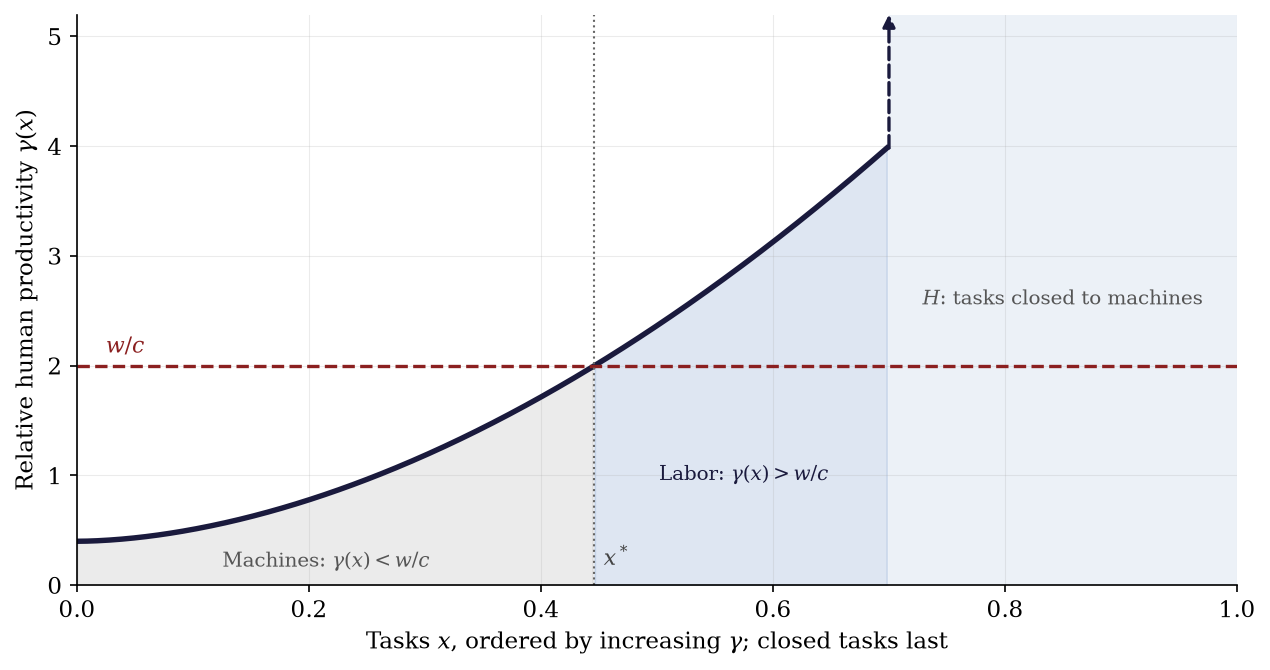
\includegraphics[width=0.88\linewidth]{figures/fig_schedule.png}
\caption{The task-assignment schedule. Tasks are ordered so $\gamma(x)$
increases. On the machine-contestable set, the ratio $w/c$ divides tasks:
machines hold tasks with $\gamma(x)<w/c$, labor holds tasks with
$\gamma(x)>w/c$, and an interior margin $x^*$ satisfies equality. Tasks in
$H$ are closed to machines and appear as a wall at the right edge. If labor
holds no machine-contestable task, the wall marks a boundary case rather
than an additional price schedule. A cheaper machine or a lower $\gamma$
near an interior margin shifts tasks toward machines.}
\label{fig:schedule}
\end{figure}


\subsection{Pricing the machine substitute}

The task-margin condition prices labor against the machine at the marginal task. The remaining object is the machine rental $c$. A machine is itself
produced, so its price depends on the inputs required to reproduce machine
services.

Suppose one unit of machine services is produced with three kinds of inputs:
$a$ units of machine services themselves ($a<1$: machines net-reproduce);
$\lambda$ labor-hours --- the fabrication, operation, maintenance, and
installation the machine sector still buys; and $b$ units of services from a
non-produced input, such as a site or mineral deposit, renting at $r$. As a price equation this is
the one-sector version of the input-output cost systems of Leontief (1936) and
Sraffa (1960): with free entry and constant returns, the rental equals unit cost,
\begin{equation}\label{eq:recursion}
c = a\cdot c + \lambda\cdot w + b\cdot r.
\end{equation}

The first term is recursively embodied machine content; the second is the wage
bill inside the substitute; the third is the claim on the inputs at which the
recursion terminates. We call this backward tracing of the machine rental
through its own input costs the \emph{machine-sector cost recursion}, below
simply the recursion. Call an input \emph{terminal over a horizon} when its
supply cannot expand through the production process within that horizon;
the propositions say ``non-produced'' for inputs outside the production
recursion. Land is a lasting example; produced bottlenecks such as grid
connections or fabrication capacity may be terminal only temporarily.
Electricity, structures, and extraction are produced activities whose costs
are traced through the recursion. The scalar model follows one non-produced
input: $r$ is its service rental, $b$ the services required per unit of machine
output, and $T$ its fixed service endowment per period. Several inputs carry
separate rentals in Appendix~\ref{app:environment}. We reserve \emph{pure rent}
for income due to fixed supply and \emph{site rent} for the land component of
real-estate income, excluding structures. The results hold over horizons on
which the specified service endowments are fixed; long-run applications require
persistent non-produced inputs.


\subsection{Closing the replacement price}

The task margin and the machine-sector price equation form a closed system. The
first prices labor against the substitute; the second prices the substitute
against its own inputs.

\begin{proposition}[replacement closure]\label{prop:replacement}
Let the task margin hold,
\[
w = c\cdot\gamma(x^*),
\]
and let machine services be priced by free entry,
\[
c = ac + \lambda w + br.
\]
If $1-a-\lambda\gamma(x^*)>0$, then
\begin{equation}\label{eq:closure}
c =
\frac{b\cdot r}{1-a-\lambda\gamma(x^*)},
\qquad
w =
\frac{\gamma(x^*)\cdot b\cdot r}
     {1-a-\lambda\gamma(x^*)}.
\end{equation}

The wage is a claim on terminal rents, scaled by relative productivity at the
assignment margin and amplified by the production recursion. On the viable set
both prices rise in $\lambda$ and in $\gamma(x^*)$.
\end{proposition}

\begin{proof}
Substitute $w=c\gamma(x^*)$ into the zero-profit condition:
\[
c = ac + \lambda c\gamma(x^*) + br,
\]
so
\[
c\cdot(1-a-\lambda\gamma(x^*)) = br.
\]
Multiply by $\gamma(x^*)$ for the wage. The derivatives are
\[
\frac{\partial w}{\partial\lambda}
=
\frac{\gamma(x^*)^2br}
     {(1-a-\lambda\gamma(x^*))^2},
\]
and
\[
\frac{\partial w}{\partial\gamma(x^*)}
=
\frac{br(1-a)}
     {(1-a-\lambda\gamma(x^*))^2},
\]
both positive; and
\[
\frac{\partial c}{\partial\gamma(x^*)}
=
\frac{\lambda br}
     {(1-a-\lambda\gamma(x^*))^2},
\]
positive exactly when $\lambda>0$.
\end{proof}

The viability condition has an intuitive reading:
$a+\lambda\gamma(x^*)$ is the produced content of one unit of machine services
once its labor is priced at the task margin --- direct machine content $a$, plus
the machine-equivalent $\lambda\gamma(x^*)$ of its labor. If that reaches one,
the sector cannot deliver services at any finite price.


\subsection{Two margins of automation}

The closure separates two kinds of automation that are usually discussed as one.

\textbf{Task automation} lowers $\gamma(x^*)$: machines improve at tasks near the
assignment margin, so a marginal human hour replaces less machine service. This
is the automation margin of the task literature.

\textbf{Recursive automation} lowers $\lambda$: fewer human hours are required to
produce, operate, and maintain machine services themselves. This removes the wage
bill from the substitute's own cost base and therefore lowers the replacement
price directly. 

Either change lowers the wage supported by a given terminal rent. And they
interact: with $\lambda>0$, task automation also cheapens the machine, because it
cheapens the machine sector's own labor.

A worked instance shows the recursion's amplification. At
\[
(a,\lambda,\gamma(x^*),b,r)=(0.5,0.1,3,0.2,1),
\]
the recipe gives $c=1$ and $w=3$, and one checks
\[
1 = 0.5\cdot1 + 0.1\cdot3 + 0.2\cdot1.
\]
Now let recursive automation run $\lambda$ from 0.1 to 0, holding everything
else fixed. Then $c$ falls to 0.4 and the wage falls to 1.2 --- a 60\% reduction
from removing one tenth of an hour of labor from the machine recipe, because
that tenth of an hour, priced at the margin wage, was 30\% of the recipe's cost.

In the limit $\lambda\to0$,
\begin{equation}\label{eq:lambda-zero}
c \to \frac{b\cdot r}{1-a},
\end{equation}
and the replacement price contains no wage at all: its reproducible components
are internal to the recursion, and what remains in unit cost is the claim on the
terminal input. Time preference and durability add an interest term to the
recursion but do not change the conclusion; Appendix~\ref{app:environment} has
the derivation, along with the matrix version for many machine types and several
terminal inputs.

\textbf{Ideas are the boundary case.} An idea's reproduction requires
approximately nothing of anything. so its competitive price is approximately zero. Any positive
price on an idea is institutional scarcity, chosen because at marginal-cost
pricing, ideas with fixed creation costs are not created (Romer 1990).
Institutional rents are therefore real, revocable, and policy-elastic; the income accounting in Section~\ref{sec:limit} treats them as additional claims when they are present, rather than identifying them with physical scarcity.

\section{The outside option: pricing exit}\label{sec:floor}

The firm-side condition supplies labor's replacement value. Participation supplies the other side: a worker accepts when the wage reaches the outside option $s$. For long-run technological change, treating $s$ as fixed hides the relative price of the consumption required outside market work.

Exit is a consumption problem. A person who leaves the labor market lives on
household production, family, savings, transfers, informal work, a plot --- and
every one of those arrangements uses housing, space, energy, food, and care.
Field evidence prices the components: the value of non-work time and household
production is substantial and heterogeneous (Mas and Pallais 2019), and the
calibration that resolves the volatility puzzle sets the aggregate outside
option high for exactly this reason (Hagedorn and Manovskii 2008). If the inputs
of unwaged life become expensive relative to goods, the value of exit falls with
no change in anyone's capabilities.

Model the exit life directly. Let $q = r/p$ be the price of non-produced services relative to the goods price $p$ (the machine-made good is the numeraire below). An independent exit arrangement yields a gross exit value $s_0$ in goods units and requires $h_e$ units of the non-produced input's services. Land provides a concrete example: the requirement is quality-adjusted access to space, so no particular parcel is needed. If independent access is unaffordable, exit degrades to a dependency floor $\underline{s} < s_0$. In the housing example, this means access through someone else's household, in the modern economy often a parent's spare room. So
\begin{equation}\label{eq:exit}
s(q) = \max( s_0 - q\cdot h_e , \underline{s} ),
\end{equation}
falling one-for-one with $q\cdot h_e$ until the dependency floor binds; thereafter, further rent increases do not reduce $s$. We call $s(q)$ the \emph{participation floor}: the value, in goods units, of not supplying the market hour. The functional form is deliberately minimal; the only essential property is $\partial s/\partial q \le 0$. An exit bundle that also contains produced goods adds a goods term whose relative cost falls with automation. The bundle retains a direct requirement for non-produced services: supplying one's own hours still requires access to the site on which to live, alongside the resources embodied in food and energy.

\begin{proposition}[the endogenous outside option]\label{prop:exit}
In the land-access example: (i) While suitable parcels lie idle --- parcels on which the gross exit value $s_0$ is attainable --- the marginal such parcel rents at zero: the exit plot is free and $s = s_0$. An unpriced margin of this kind is what ``a commons'' is, economically: idle land, family access, public provision --- any arrangement supplying the scarce input below its rental price. (ii) Once no suitable parcel lies idle, the exit plot pays the ruling rent and $s = s(q)$ above. The trigger is the exhaustion of suitable idle land. (iii) For workers with $\partial s/\partial q < 0$, a rise in $q$ shifts labor supply outward: participation weakly rises, and by Proposition~\ref{prop:margin}(ii) the equilibrium wage weakly falls where the schedule has slope holding the labor-demand schedule fixed. The full equilibrium effect also includes the response of replacement costs and output.
\end{proposition}

\begin{proof}
(i) Any positive rent on the marginal parcel is undercut by an idle neighbor of reservation rent zero. (ii) With no idle neighbor, the exit plot must outbid other uses for the marginal suitable parcel, whose rent is now positive; the net exit value is $s_0 - q\cdot h_e$ until $\underline{s}$ binds. (iii) A lower reservation value moves the participation step down: more workers accept at any wage; the wage response is Proposition~\ref{prop:margin}'s comparative statics.
\end{proof}

A parcel rents at zero because little can be done with it --- which is why the truly idle margin supports no exit either. Free and livable together is a particular historical configuration. When no suitable parcel idles, the dependency floor $\underline{s}$ is not land-free but otherwise-funded, in three modern forms. Dependency: a room supplied out of someone else's wage or ownership, an unpaid transfer from the employed to the exited. Public provision: the out-of-work payment of Appendix~\ref{app:conditionality}, unconditional in few places and limited in scope where it exists. Tolerated use: living on land one does not hold, its price paid in eviction risk rather than rent. Each is a commons in the degraded sense: the scarce input supplied below its rent, from someone's budget, the state's, or the law's forbearance. None is insulated from $q$: the host's capacity to share inherits the host's rent bill, so the flat segment at $\underline{s}$ is an upper bound.

This is the model's understanding of enclosure. Close the idle margin --- by law, as in the historical enclosures, or by price, as when housing scarcity does the same work parcel by parcel --- and three things happen at once: the outside option falls, participation rises, and the wage falls at given technology. Enclosure therefore expands labor supply. Marx said so as history; Lewis (1954) built the two-sector version, with the traditional sector's per-head product as the modern sector's wage anchor; Polanyi (1944) documented the institutional campaign. The mechanism is visible in rent-to-wage ratios, household formation, and coresidence. Appendix~\ref{app:race} analyzes the timing between the closing of this margin and the arrival of a funded replacement.

\section{The two sides of the wage}\label{sec:interval}

The two closures can now be assembled. On the labor-demand side, competitive
assignment requires
\[
w = c(r)\cdot\gamma(x^*)
\]
at an active machine-contestable margin. On the labor-supply side,
participation requires
\[
w \ge s(q), \qquad q=r/p.
\]
The first is an equilibrium equality at
an interior task margin; the second is a participation constraint. Terminal
scarcity nevertheless enters both:
\[
r
\to c(r)
\to c(r)\gamma(x^*)
\to \textit{labor demand},
\qquad
q=r/p
\to s(q)
\to \textit{labor supply}.
\]

The two channels can pull the equilibrium wage in opposite directions. A higher
terminal rent makes the machine substitute more expensive and therefore raises
the replacement value of labor at a given assignment margin. The same rise in
rent can erode the outside option, expand participation, and move the assignment
margin in the opposite direction. Which effect dominates is a parameter
question. What is not ambiguous is that both sides are formed partly in the
market for non-produced inputs.

In bargaining language, the same objects delimit the surplus
available for bargaining: the value generated by employing labor relative to
the firm's alternative, and the value of work relative to the worker's
alternative. The present competitive benchmark selects the wage through the
task-assignment condition, while participation determines who enters and
therefore where the assignment margin settles. Institutions can insert wedges
between those objects, but need not supply their underlying levels.

Automation can shift both sides: task and recursive automation lower the replacement value at a given margin, while a higher $q$ can lower the reduced-form outside option. Participation then helps determine which task is marginal. The wage response depends on the local schedule, the machine recipe, and output demand.

\textbf{Heterogeneity and skill premia.} Workers differ in productivity across tasks and in their outside options. For each type, an active machine-contestable margin prices the wage against the machine substitute. When a type works only at tasks in $H$, its wage depends on demand for those services, the supply of that type, institutions, and participation. The outside option supplies a lower bound; statements about the dependency floor concern the bottom of the support. Relative wages also reflect comparative advantage and substitution between worker types, together with their relative supplies. Training takes time and resources to acquire. Where entry into training is open, those costs discipline the long-run premium, while a shortage of trained workers can sustain a higher return. These comparisons guide the historical discussion; a full account of skill premia would jointly determine task assignment, training, and labor supplies.

\section{Purchasing power at an interior margin}\label{sec:limit}

At an active task margin, the replacement closure determines the wage relative to the rental of the non-produced input:
\begin{equation}\label{eq:fork-price}
\frac{w}{r}=\frac{b\gamma(x^*)}{1-a-\lambda\gamma(x^*)}.
\end{equation}
At a given marginal task, a fall in $\gamma(x^*)$ or in $\lambda$ lowers this ratio, holding the other recipe coefficients fixed. In equilibrium the margin can move as well. The relevant empirical object is therefore the cost of replacing labor that remains employed, not average machine capability across all tasks.

\subsection{Category costs and wage purchasing power}

Let category $j$ require $b_j\ge0$ units of services from the non-produced input directly, alongside a task list $\mathcal X_j$. This direct requirement is unavoidable under either human or machine assignment. Each task has a feasible human method, and
\[
\bar L_j=\int_{\mathcal X_j}\frac{dx}{\gamma_{Lj}(x)}\in(0,\infty)
\]
is the hours required to perform that list entirely by human labor. It is a technological alternative, not the hours actually employed. Task quantities are included in the integration measure; produced inputs other than the machine services priced by $c$ are traced into the task list. The machine sector's inputs are already priced in $c$ and are not counted again. A category can have $b_j=0$ while using the non-produced input indirectly through its machine supply chain.

At an active margin, $c/w=1/\gamma(x^*)$. Express each category's task cost in units of the wage:
\begin{equation}\label{eq:effective-hours}
L_j^*=\int_{\mathcal X_j}\frac{1}{\gamma_{Lj}(x)}
\min\left\{1,\frac{\gamma_j(x)}{\gamma(x^*)}\right\}dx,
\qquad \gamma_j(x)=\frac{\gamma_{Lj}(x)}{\gamma_{Mj}(x)}.
\end{equation}
On a human-required task the minimum is one. $L_j^*$ is the wage-equivalent cost of the task list, including machine work; it is not a count of human hours. It depends on the task technologies and the equilibrium margin, and satisfies $0\le L_j^*\le\bar L_j$.

\begin{proposition}[the real-wage fork at an interior margin]\label{prop:fork}
With an active replacement margin and the category requirements above, competitive prices satisfy
\begin{equation}\label{eq:composites}
p_j=wL_j^*+rb_j,\qquad
\frac{w}{p_j}=\frac{1}{L_j^*+b_j(r/w)},\qquad
\frac{r}{w}=\frac{1-a-\lambda\gamma(x^*)}{b\gamma(x^*)}.
\end{equation}
For arbitrary cost-minimizing task assignments, including boundary assignments, the prices also obey
\begin{equation}\label{eq:category-bounds}
rb_j\le p_j\le rb_j+w\bar L_j.
\end{equation}
Consequently, when $b_j>0$,
\begin{equation}\label{eq:fork-pair}
\frac{1}{\bar L_j+b_j(r/w)}
\le\frac{w}{p_j}
\le\frac{w/r}{b_j}.
\end{equation}
When $b_j=0$, wage purchasing power satisfies $w/p_j\ge1/\bar L_j$.
\end{proposition}

\begin{proof}
The competitive category price is
\[
p_j=rb_j+\int_{\mathcal X_j}
\min\left\{\frac{w}{\gamma_{Lj}(x)},
            \frac{c}{\gamma_{Mj}(x)}\right\}dx,
\]
where machine cost is infinite on tasks closed to machines. At an active margin, dividing each task cost by $w$ and substituting $c/w=1/\gamma(x^*)$ gives $L_j^*$ and \eqref{eq:composites}. Every task cost is nonnegative and no larger than the human method's cost. Integrating gives \eqref{eq:category-bounds}; dividing and inverting gives \eqref{eq:fork-pair} and the case $b_j=0$.
\end{proof}

The upper bound comes from the rent bill: an hour's wage buys $w/r$ units of the non-produced input's services, and a unit of category $j$ requires at least $b_j$ units. The lower bound is the feasible human method. Machine substitution can make a category cheaper than that method, raising purchasing power above the lower bound. The quantities measure what wages buy; ownership income and transfers also fund consumption.

The exact formula separates the wage-equivalent task cost $L_j^*$ from the direct rent bill $b_j(r/w)$. At given $L_j^*$ and $b_j>0$, a rise in $r/w$ lowers wage purchasing power; at given $r/w$, a fall in $L_j^*$ raises it. Both can move under automation, so the net change depends on task technologies, movement of the margin, and direct input requirements. The ratio $b_j/\bar L_j$ measures the non-produced input requirement per hour of the feasible human method and describes the lower bound's sensitivity to $r/w$. Ordering actual category price changes also requires information about their task costs.

\begin{corollary}[a vanishing wage--rent ratio]
Along a sequence of equilibria with an active replacement margin, suppose
\[
b\gamma(x^*)\to0,\qquad
1-a-\lambda\gamma(x^*)\ge\varepsilon>0.
\]
Then $w/r\to0$. Wage purchasing power tends to zero for every category whose direct requirement for the non-produced input stays bounded away from zero. For a category with no direct requirement, a uniform upper bound on $\bar L_j$ preserves a positive lower bound on wage purchasing power.
\end{corollary}

\begin{proof}
Equation~\eqref{eq:fork-price} gives $0<w/r\le b\gamma(x^*)/\varepsilon\to0$. If $b_j\ge\underline b_j>0$, Proposition~\ref{prop:fork} gives $0<w/p_j\le(w/r)/\underline b_j\to0$. Its bound for $b_j=0$ gives the final statement.
\end{proof}

The sufficient conditions concern replacement at the equilibrium margin. At fixed positive $\gamma(x^*)$ and $b$, sending $\lambda$ to zero leaves a positive wage--rent ratio, $b\gamma(x^*)/(1-a)$. The path therefore depends on both the machine recipe and relative capability at the tasks labor still holds. Human-required work can sustain a boundary assignment, and falling direct requirements for non-produced inputs can sustain a category's wage purchasing power. Appendix~\ref{app:equilibrium} gives a complete equilibrium with a strictly increasing schedule and an illustrative sequence with a persistent two-to-one capability ratio.

\textbf{Flat-case remark.} If relative capability is constant at $\bar\gamma$ across a category's tasks and $w=c\bar\gamma$, every task is at cost parity and $L_j^*=\bar L_j$. The upper price bound is then attained:
\[
p_j=w\bar L_j+rb_j,\qquad
\frac{w}{p_j}=\frac{1}{\bar L_j+b_j(r/w)}.
\]
The category's real wage is exactly $1/\bar L_j$ when $b_j=0$; a higher ratio $b_j/\bar L_j$ makes the rent term dominate sooner as $r/w$ rises.

\subsection{Factor income while labor remains employed}

\begin{proposition}[income accounting]\label{prop:income}
In the competitive flow economy with human hours and one non-produced input as the two primary factors, let $N_a\le N$ be total employed hours, including labor in machine production, and let $T$ be the fixed, fully employed service endowment of the non-produced input. Final expenditure and factor income satisfy
\begin{equation}\label{eq:income}
I=wN_a+rT,\qquad
\frac{wN_a}{I}=\frac{(w/r)N_a}{(w/r)N_a+T}.
\end{equation}
At given $N_a$ and $T$, a lower wage--rent ratio lowers labor's share. With bounded total hours and fixed $T>0$, $w/r\to0$ implies that labor's share tends to zero.
\end{proposition}

\begin{proof}
Intermediate payments cancel when final expenditure is traced through the machine sector's zero-profit condition, leaving the payments for all human hours and non-produced services. Appendix~\ref{app:accounting} gives the cancellation explicitly. Divide by $r$ for the share formula; bounded hours give the limit.
\end{proof}

Ownership of the non-produced input receives the non-wage component of income in this two-factor flow benchmark. The wage bill includes work at final tasks as well as in machine production; setting $\lambda=0$ leaves final-task wages in the income identity. Interest, institutional rents, and transitional capacity rents add income components outside this benchmark. Labor's share responds jointly to the wage--rent ratio and employment, so increased employment can offset a local fall in $w/r$.

\section{Distribution: rent taxation and a uniform transfer}\label{sec:fiscal}

The income identity separates two sources of purchasing power: hours sold and ownership claims. A lower wage--rent ratio increases the importance of ownership at given employment. Rent taxation and transfers determine how this income is distributed across households.

Let non-produced inputs supply fixed service endowments $T_j$ at gross competitive rents $r_j$, and write $R=\sum_jr_jT_j$. A tax at rate $\tau_R$ on pure ownership rents finances a uniform per-person transfer $d=\tau_RR/N$, paid identically in and out of work.

\begin{proposition}[sharing rents while labor remains employed]\label{prop:welfare}
(i) A tax on the pure ownership rent of a fixed factor does not change its physical supply. Producers continue to face the gross rental for using it; the ownership tax introduces no direct wedge between their cost and that rental.

(ii) An unconditional transfer has no withdrawal at the work--exit boundary: the transfer differential between working and not working is zero. In the reduced-form participation comparison with a fixed reservation value, the common payment cancels. Household participation can also respond through income effects.

(iii) If person $i$ owns shares $\omega_{ij}$ of the terminal stocks and supplies $n_i$ hours at wage $w$, receipts are
\[
y_i=wn_i+(1-\tau_R)\sum_j\omega_{ij}r_jT_j+\tau_RR/N.
\]
At given gross prices and hours, aggregate receipts are $wN_a+R$, and the tax redistributes the rent component toward an equal per-person allocation.
\end{proposition}

\begin{proof}
(i) The taxed stock is fixed by assumption, and its user pays the gross rental regardless of the owner's after-tax receipt. (ii) Subtract the same payment from the resources in work and exit. (iii) Sum over people, using $\sum_i n_i=N_a$ and $\sum_i\omega_{ij}=1$ for every stock.
\end{proof}

Redistribution can change demand, rents, and willingness to work. For example, with utility $\log g-\chi n$ and positive goods-unit resources $A$ in exit, a common transfer $d$ raises the reservation wage to $(e^\chi-1)(A+d)$: the additional resources allow the person to refuse more work. This income effect coexists with a zero benefit-withdrawal differential. The policy's allocation effects therefore depend on household preferences, ownership, and equilibrium prices.

A wage-funded transfer draws on the labor market as both a financing base and a participation margin. Its incidence depends on demand and supply elasticities. Appendix~\ref{app:fiscal} states the local incidence comparison and the conditions under which the rent base can cover a subsistence bundle. The fiscal lineage is George (1879); the Henry George theorem of Arnott and Stiglitz (1979) is related but distinct.

\section{History as four configurations of the model}\label{sec:history}

The model can be applied to the long record as four configurations of the relative-productivity schedule (Figure~\ref{fig:eras}). Because schedules may differ across worker types, the figure shows each configuration for both an untrained entrant and a worker with accumulated training or experience. The comparison is interpretive: the baseline model does not separately solve for the two wage schedules or for investment in training.

\begin{figure}[t!]
\centering
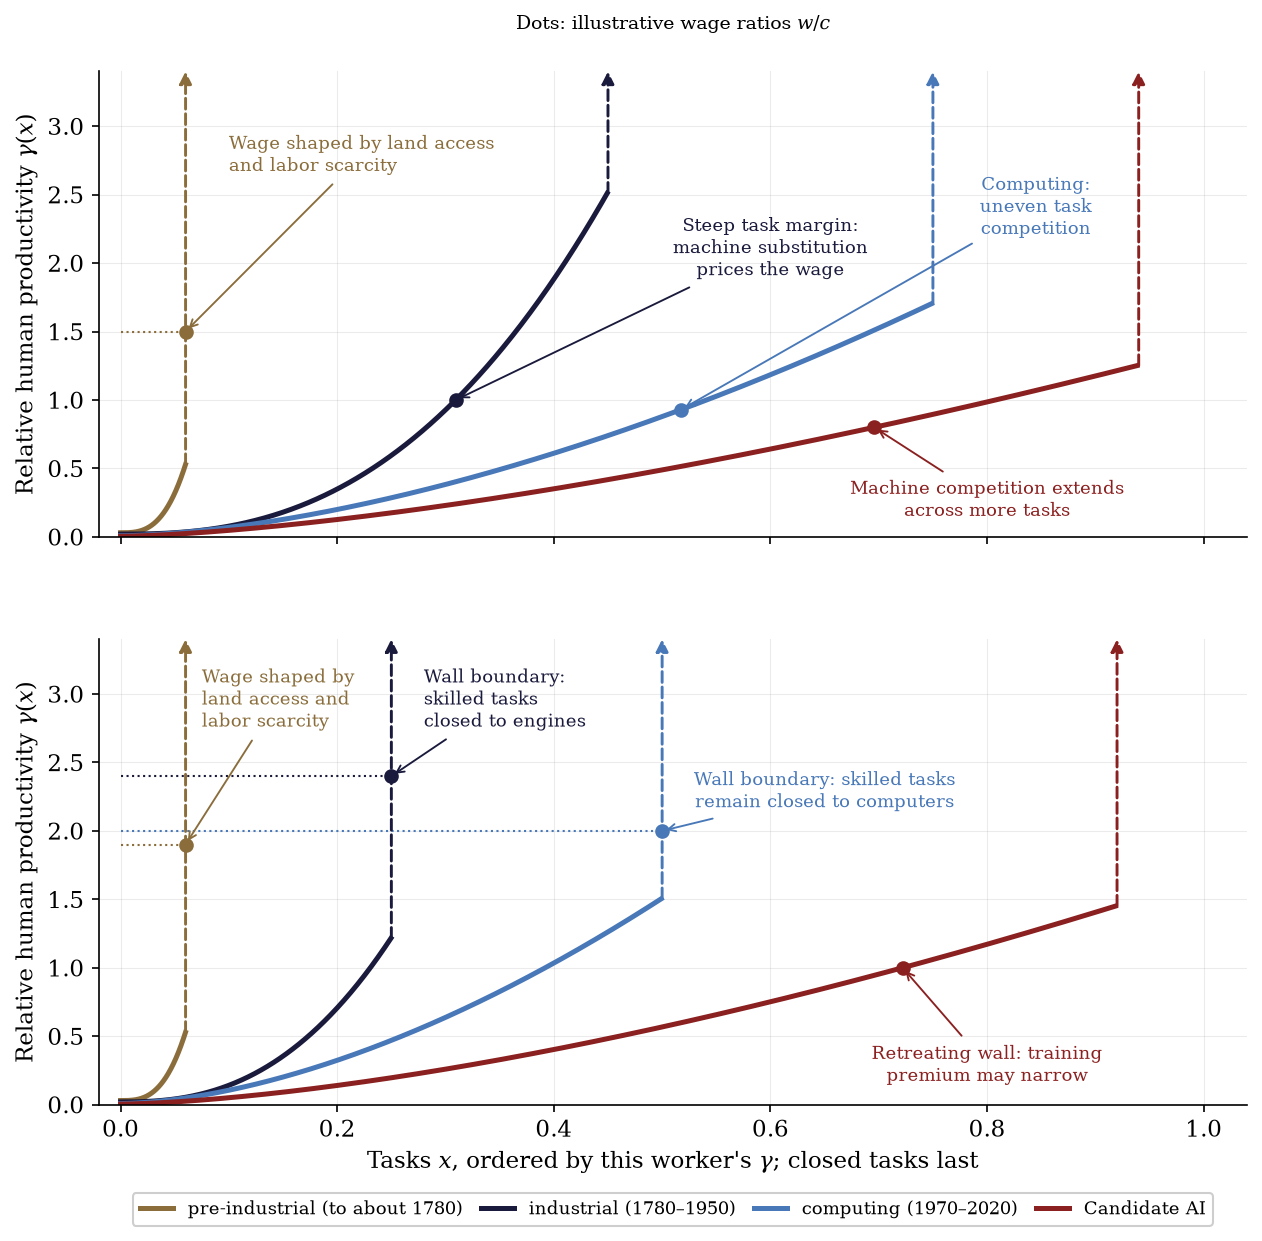
\includegraphics[width=0.88\linewidth]{figures/fig_eras_workers.png}
\caption{Four schematic configurations of the task schedule, shown for
an untrained entrant (top) and a worker with accumulated training or experience
(bottom). Each panel uses a different worker-specific task mix, held fixed
across eras within that panel; differences in wall location reflect these
mixes, not an effect of training on machine capability. Closed tasks appear as
a wall at the right edge. Dot heights are illustrative wage--machine-rental
ratios $w/c$, not purchasing power over goods or non-produced services. A dot on the
contestable schedule marks an interior margin satisfying $w/c=\gamma(x^*)$;
a dot on the wall marks the absence of such a margin and does not imply a
binding participation constraint. Industrialization opens physical tasks;
computing extends competition into cognitive tasks while many trained tasks
remain closed. Relative human advantage continues to vary across the open
task range. In the candidate AI configuration, machine competition extends
across more tasks, while the schedules keep rising and retain an illustrative
positive training premium. The chosen curvatures illustrate differences in
relative capability across tasks.}
\label{fig:eras}
\end{figure}

\textbf{Pre-industrial: land access and labor scarcity.} With machines scarcely present, nearly every task is closed to them; the margin sits at the wall for entrant and master alike, so the machine prices no one's hour. Demand for human services, labor scarcity, institutions, and participation then determine wages. A configuration with wages near the outside option additionally invokes demographic adjustment, with the outside option tracking access to land --- the world Ricardo and Malthus wrote down, and the one the new long-run estimates describe: pre-industrial English real wages strongly shaped by population and land, with productivity growth beginning well before wages escaped Malthusian pressure (Bouscasse, Nakamura, and Steinsson 2025). The classical account is one configuration of our model. The entrant is the farm servant hired by the year; the trained worker is the craftsman after a seven-year apprenticeship, whose premium over the servant is the cost of those years, recovered.

\textbf{Industrial: comparative advantage widens.} The Industrial Revolution created a large and uneven productivity gap across tasks: engines were far better than muscle at physical tasks but ineffective at cognitive ones. The schedule became enormously dispersed and steep. It did so for the entrant first: the young mill hand or hand-loom weaver held the tasks engines were reaching one by one, and the margin sat on the steep stretch, where what the engine cost at the next task priced the hour. The trained worker, the millwright, the engineer, the clerk, held tasks closed to engines; that margin stayed at the wall, so no machine set the wage, and it was instead a scarcity price on trained hands and heads, kept scarce by the years the training took. That dispersion opened high-productivity tasks to labor and could support a higher wage; by Proposition~\ref{prop:margin}(ii), steepness also makes employment less responsive to a given wage change and the wage more responsive to shifts in labor supply. Meanwhile machine production itself remained labor-intensive: in the recursion, both $\gamma (x^*)$ and $\lambda$ supported the wage. The escape was neither immediate nor smooth --- real wages grew slowly in the early decades as capital deepening and urbanisation preceded substantial wage growth (Crafts 2022).

\textbf{Post-industrial: machine competition broadens.} Computerization reached the simple-cognitive region of the schedule --- the routine-task evidence of Autor, Levy, and Murnane (2003) and the polarization it produced (Autor and Dorn 2013) are the cross-sectional trace. The entrant is the young clerk, cashier, or assembler whose routine tasks software and machines reached at similar cost: an interior machine-contestable margin could price the wage on a schedule of uneven relative capability. The trained worker, the developer, the physician, the engineer, held tasks computers could not: the margin stayed at the wall, and the premium for training was what the period's expansion of higher education chased. AI is a candidate extension of machine competition to further tasks, including those previously closed to machines. It may also reduce $\lambda$, the labor inside the machine sector itself. As trained tasks become contestable, skill premia depend on the replacement costs and labor supplies of the different worker types. The interior result connects these replacement costs to wage purchasing power.

\section{Measurement}\label{sec:measurement}

In this section we observe three empirical objects: the real-wage fork, the size of the rent base relative to the cost of a subsistence bundle, and the separation between the origin of consumption finance and the human effort embodied in production.

\textbf{The fork.} Over 1964--2024, the durables-to-shelter real-wage ratio reaches $4.8\times$ (Figure~\ref{fig:fork}). This descriptive comparison is consistent with the distinction in Proposition~\ref{prop:fork} between task costs and persistent requirements for non-produced inputs. Identifying the underlying task schedules and attributing the price changes requires additional task-level evidence. Food lies between the endpoints. Deflated by the food CPI, the same paycheck rose 13 percent over 1964--2024, compared with 277 percent for durables and a decline of 21 percent for shelter. The intermediate result is consistent with a category that combines direct acreage with processing labor and rising yields. Energy can be seen to be volatile, likely as world oil prices dominate the series, making it a measure of shocks rather than a trend.

\begin{figure}[t!]
\centering

\includegraphics[width=0.88\linewidth]{figures/fig_deflator_fork.png}
\caption{U.S. average hourly earnings for production and nonsupervisory
workers deflated by the consumer-price indexes for durables, food, energy,
and shelter, 1950 = 100, through the last complete calendar year, 2024.
Values before 1964 use the spliced wage series. The energy index begins in
1957; its 1950--1956 values are a linear backcast estimated over 1957--1966.
Over 1964--2024 the ratio of the durables-deflated to the shelter-deflated
wage reaches $4.8\times$, a ratio that does not depend on the index base.}
\label{fig:fork}
\end{figure}

\textbf{The floor's coverage.} The coverage ratio $\kappa$ is the fraction of one subsistence bundle that a full tax on site rents could finance per person. Figure~\ref{fig:kappa} measures aggregate site-rent flow against population times a costed subsistence bundle. The 2025 estimate is $\kappa=0.33$ [0.18--0.59], up from roughly 0.05 in the 1950s. The measures are intended as lower-bound constructions, and the physical ceiling remains land per head.

\begin{figure}[t!]
\centering
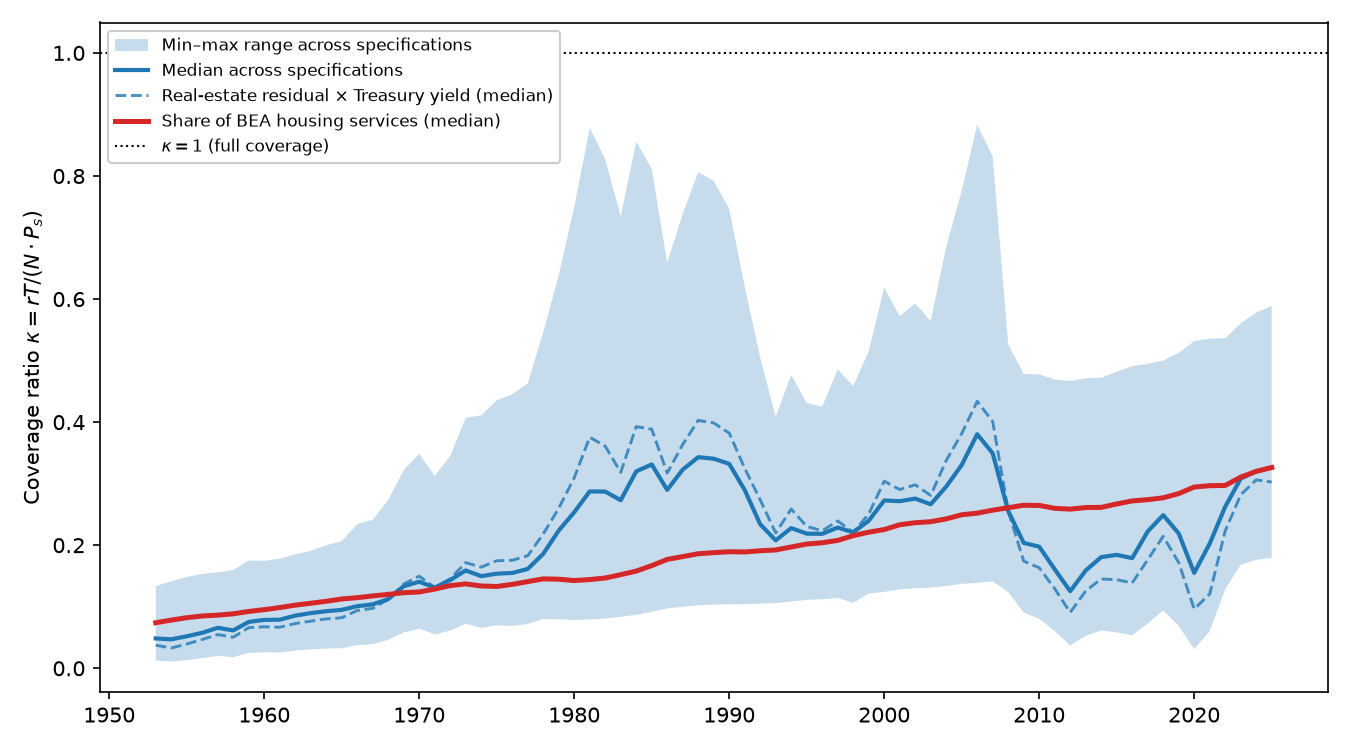
\includegraphics[width=0.88\linewidth]{figures/fig_kappa_measurement.png}
\caption{The coverage ratio $\kappa=rT/(N\cdot P_s)$ is aggregate site-rent flow divided by the cost of providing the specified subsistence bundle to every person; U.S., 1953--2025. The
line is the median and the band is the min--max range across specifications
combining land sources, capitalization rates, and subsistence bundles. The
dashed specifications subtract residential structures at replacement cost
(Z.1, BOGZ1LM155012665Q) from household real estate at market value (Z.1,
FRED HNOREMV) and convert the residual to an annual flow using the 10-year
Treasury yield (GS10), with a +150 basis-point variant and household and
economy-wide scopes. The red specifications apply land shares of 0.30 and
0.50 to PCE housing services (BEA, DHSGRC1A027NBEA). Every specification
uses population times the Orshansky 1963 subsistence bundle as the
denominator.}
\label{fig:kappa}
\end{figure}

\textbf{Financing versus production.} Consumption remains substantially more labor-financed than production is labor-intensive. In the common benchmark-data window, labor-origin resources finance 69.6\% of consumption in 2004 and 65.8\% in 2023, while full-chain human effort accounts for 48.9\% and 47.2\% of consumed production in the same years --- a gap of about nineteen percentage points at the end of the overlap (Figure~\ref{fig:labor-linkages}). The production account is the aggregate counterpart of the recursion: the human-effort share declines as machine-producing and machine-operating chains shed labor. Appendix~\ref{app:effort} gives the two accounts' construction and bounds.

\begin{figure}[t!]
\centering
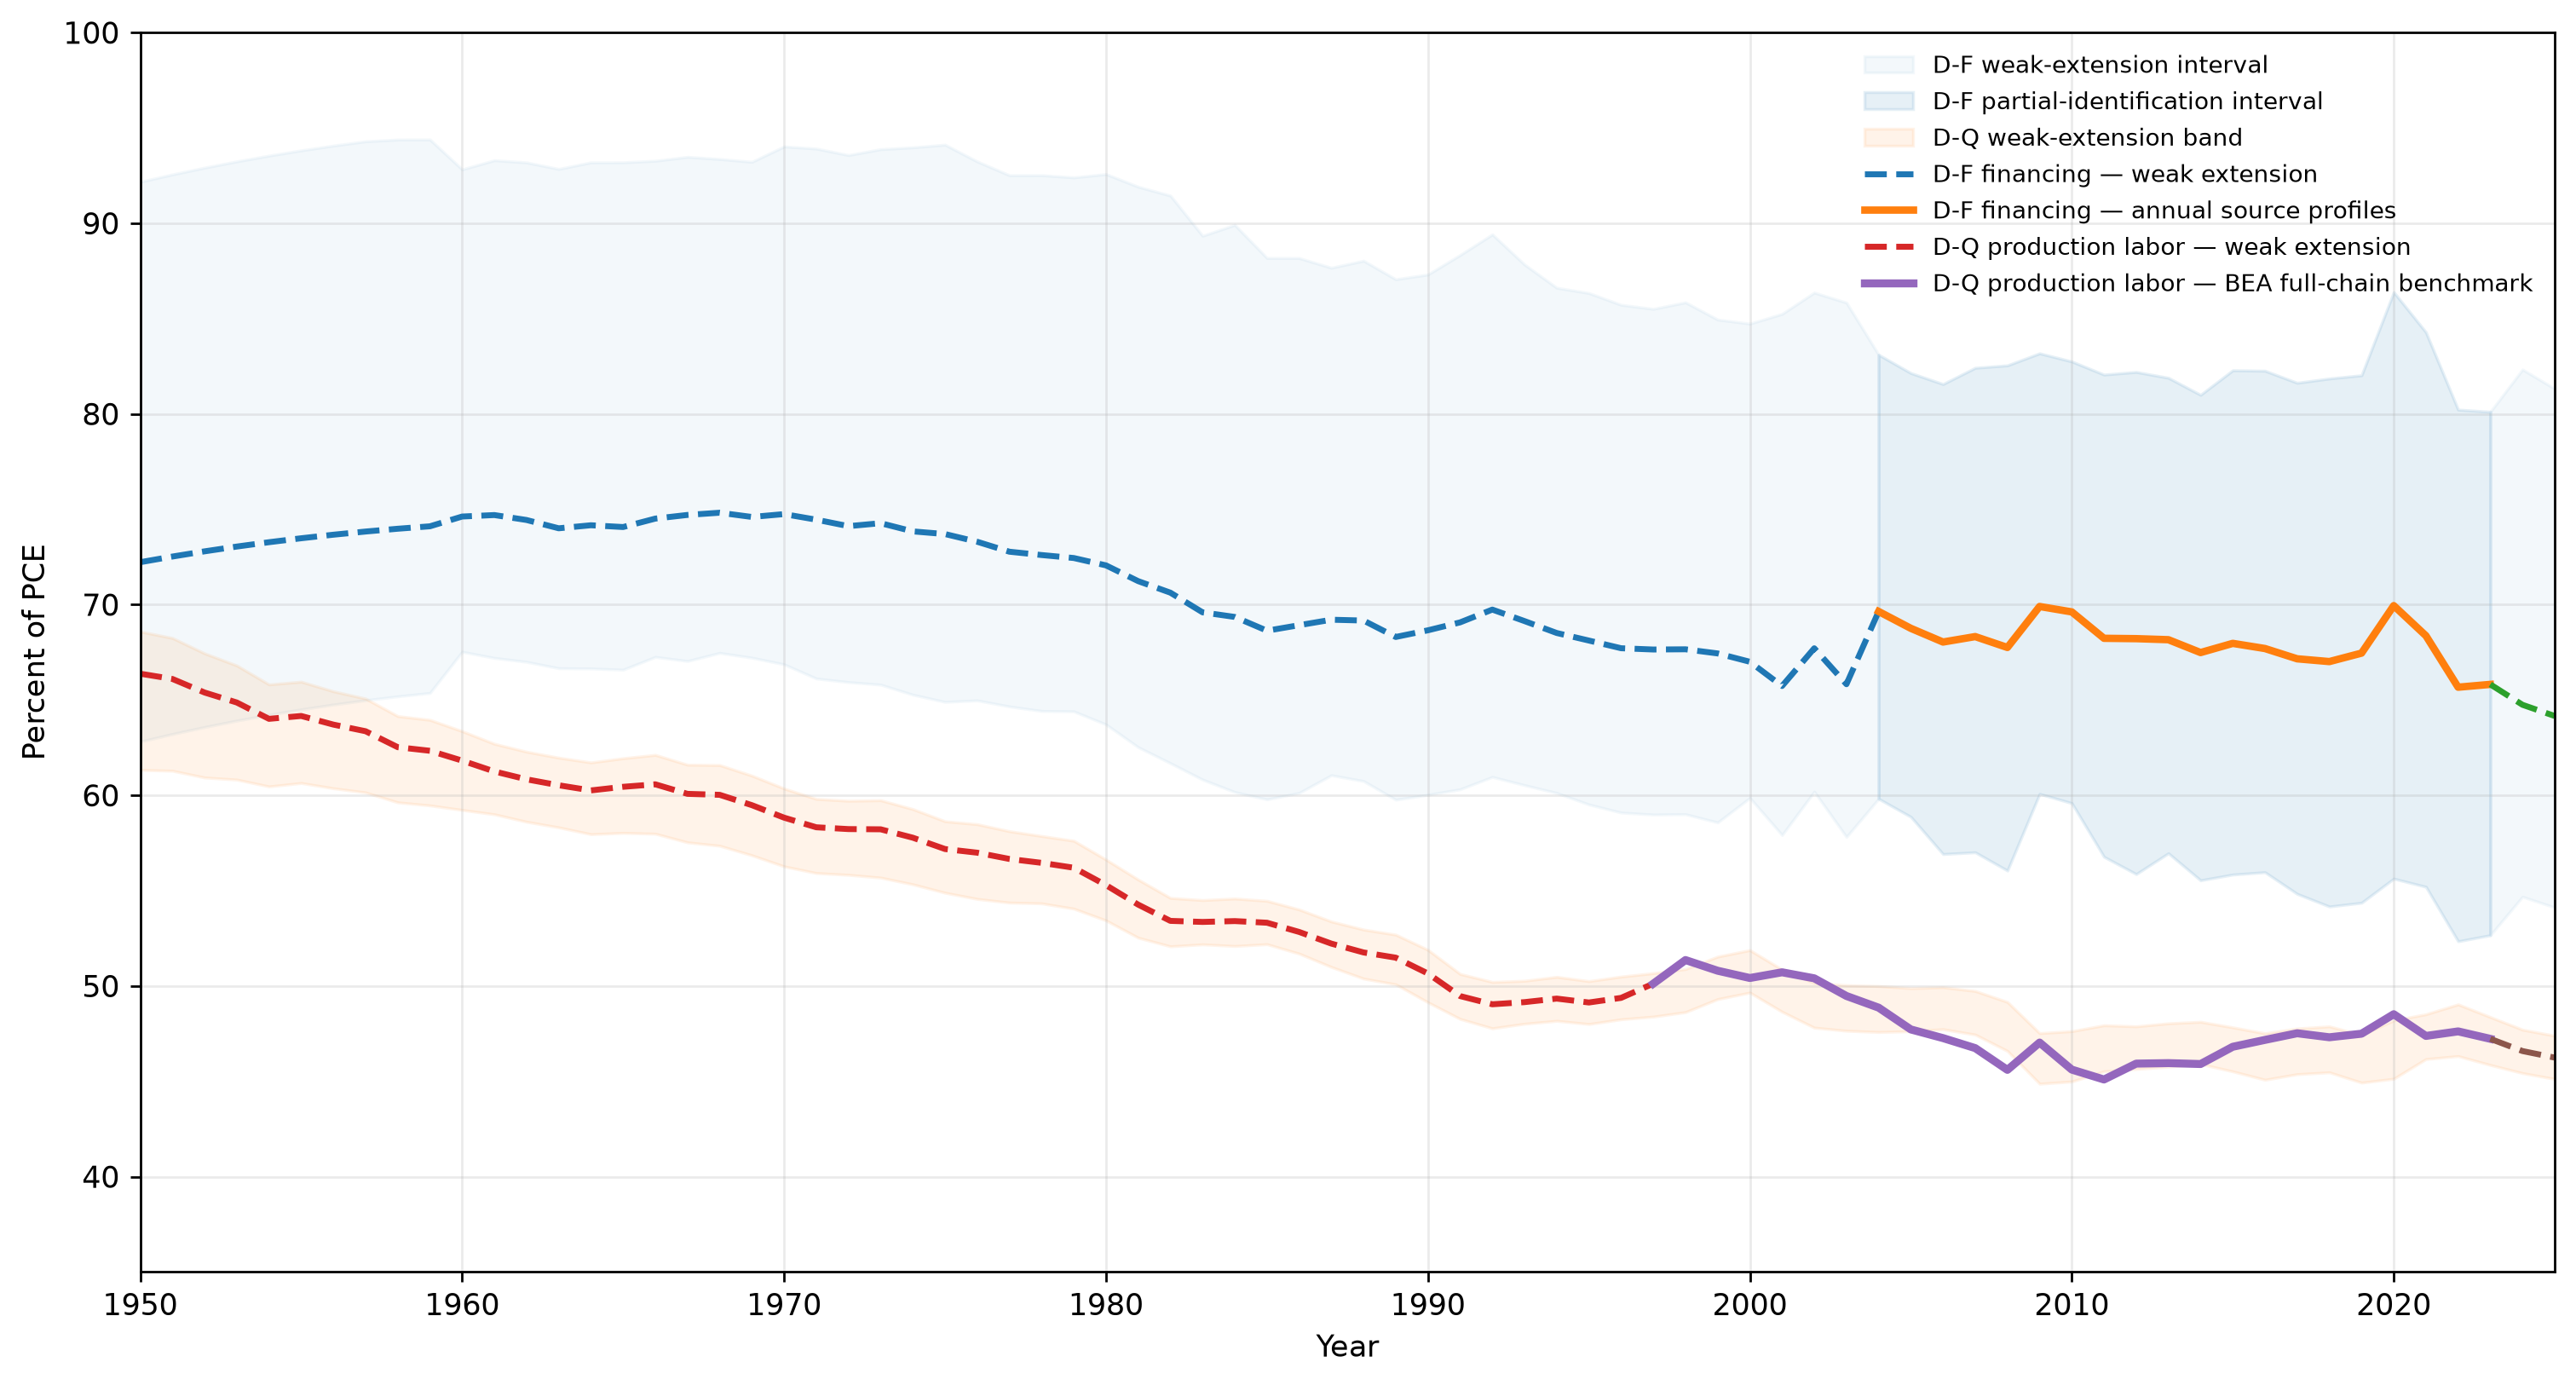
\includegraphics[width=0.92\linewidth]{figures/fig_consumption_financing_and_human_effort.png}
\caption{Two labor linkages in U.S. consumption, 1950--2025. The upper
series is the share of consumption financed from labor-origin resources; the
lower is the share of consumed production that resolves into human effort
through the full production chain. Markers identify the benchmark-data
windows: annual BEA income-source profiles for financing in 2004--2023 and
the BEA full-chain production benchmark in 1997--2023. Values outside those
windows are model-based extensions. In the common benchmark-data window,
consumption is substantially more labor-financed than production is
labor-intensive.}
\label{fig:labor-linkages}
\end{figure}

\section{Possible stabilizers}\label{sec:stabilizers}

Three stabilizers can preserve wage purchasing power over scarce services, but they work through different margins. Human-required tasks can persist by preference or by law; Appendix~\ref{app:human} shows that this can preserve aggregate labor income while leaving the median worker exposed. Institutions can reserve tasks for people outright, which is quantity rather than price protection. Supply expansion --- building, densifying, powering --- works on the other side of the model by loosening the terminal-input constraint and directly lowering $q$.

The wedge result behind that distinction is Acemoglu and Restrepo's (2026). Let a task pay a premium over the base wage --- a union premium, a licensing rent, an efficiency wage --- as a multiplicative wedge $\mu (x) > 1$. Labor then holds the task only while $w \le c\cdot \gamma (x)/\mu (x)$: allocation runs on the wedge-deflated schedule, a premium raises its own task's flip priority one-for-one, and automation is directed at the best-paid versions of each job --- their targeting result, with the documented losses concentrated in the 70th--95th within-group percentiles. A wage premium therefore increases the incentive to automate the protected task; protection survives only in quantity form --- a scope-of-practice rule extended to software, an enforceable automation ban, a mandated human in the loop. Under pressure, nothing moves while the saving from flipping runs below the cost of confrontation with a legal or strike risk; past it, everything the rule covers flips at once.

\section{Implications for artificial intelligence, and conclusion}\label{sec:ai}

AI may move both automation margins at once. It can lower $\gamma(x^*)$ where models become effective substitutes at final tasks, and it can lower $\lambda$ because software generation, chip design, datacenter operation, logistics, and research are themselves part of the machine sector's labor. Either change lowers $w/r$ at a given margin and recipe; the equilibrium effect also depends on reinstatement, demand, and participation. Section~\ref{sec:limit} translates the resulting wage--rent ratio into category purchasing power through task costs and direct requirements for non-produced inputs. The path of purchasing power depends on how these components change together. If replacement at the active margin drives $w/r$ toward zero while direct requirements for the non-produced input remain bounded away from zero, wage command over those categories falls toward zero. The implications for the AI buildout concern the inputs that remain scarce: sites, power, water, minerals, and legally protected assets. Model weights are reproducible ideas; the ownership claims on the scarce services needed to use them are a separate part of the cost structure.

The relative-price mechanism also affects fiscal capacity: a rise in $q$ lowers the modeled exit option and raises the rent base in goods units. Coverage of a rent-funded subsistence transfer remains near one-third, while 0.68 of tax revenue is still raised from labor-income bases. A tax on pure fixed-factor rents can fund a payment paid equally in and out of work. Its scale, income effects, and equilibrium consequences remain empirical questions. Appendix~\ref{app:fiscal} asks how much the rent base can finance and how alternative financing changes incentives.

The remaining empirical question is whether the machine-production recursion
is paying a smaller share of cost to wages and a larger share to
terminal-input rents, and whether the same scarcity is eroding the value of
exit. Although it requires a significant re-framing of the last 70 years of world economic history, we consider the answer to be obvious.

The intuitive reading of that re-framing, and of what our paper may conjecture, is this: labor may currently be behaving as a kind of grand market distortion, and may have been doing so for many decades. Our economies have almost no mechanism to limit the supply of labor. With other goods, like oil six years ago or capital when inflation rates near zero, the economy can signal its desire to have supply lowered. However, as wages represent the majority of consumer demand, this mechanism is unavailable for labor itself. Instead, the economy dutifully creates jobs, \textit{at cost}. Either with significant wedges, the ``Bullshit Jobs`` dynamic, or near the subsistence and dependency floors, the ``gig economy``. A K-shaped graph in many of our measures of economic health then should come as no surprise. The hollowing out of our middle class, as no surprise. Youth unemployment, adult children living with their parents, and the loss of the atomic family, as no surprise. The difficulty of governments to maintain fiscal restraint, as no surprise. The stagnant growth of developed economies despite significant advances in computing, as no surprise.

This work represents in many ways the synthesis of centuries of economic thought. The classical economists may not have been wrong, they just did not know what technology could do to the wage. George was not wrong, he simply wrote his work at a time when his policies were needed the least. Keynes was not wrong, but he did not foresee the change that cognitive automation would bring. Rather, we may now be able to bring all these ideas together into a substantive wage equation.

\section{Future Work}
There is much still to be done. The model is static: it describes prices and limits, but not the path the economy takes between them. A dynamic extension could ask whether automation arrives smoothly or in waves, how quickly rents adjust, and what happens when wages fall faster than institutions can respond. It may also have implications for monetary policy. When machine-made goods become cheaper while housing, energy, and other scarce necessities become more expensive, a single inflation rate can hide significant nuances. Can one interest rate stabilize both sides of a divide? Do low interest rates support employment and demand, or do they mainly raise scarce-asset rents and accelerate the replacement of labor? The present model cannot answer these questions, but it may provide the relative-price structure needed to ask them.

The model’s implications for participation have also not been fully explored. A worsening outside option may keep people in poorly paid work because leaving becomes unaffordable, but falling wages may eventually cause others to withdraw from the labor market entirely. Adding households would open further questions. If wages buy ever more manufactured goods but ever less housing, energy, and care, then forming a household may become harder even while measured productivity rises. Delayed household formation, adult children remaining with their parents, and declining fertility may therefore reflect not only changing preferences, but a growing separation between wages and the scarce goods required to begin an independent life.

The model also suggests avenues for choosing the tax mix as automation changes the sources of income. Labor and ownership both finance consumption, and site rents may cover only part of a desired transfer. The relevant question is the best mixture of value-added, income, corporate, land-value, and other pure-rent taxes. Our input-output and consumption financing measurements may help significantly with this. Sovereign wealth funds may provide another instrument. A country with little land, energy, or mineral wealth of its own cannot tax rents earned elsewhere, but it can acquire claims on them. For resource-poor countries, owning part of the world’s scarce-resource base may eventually matter as much as taxing the domestic one.

Finally, structuring a society that no longer orbits around labor is not a trivial problem. Work provides more than a wage. It provides structure to the day, social contact, status, a sense of contribution, and an understanding of the complexity of the real economy. An income transfer can replace a wage; it cannot by itself replace all of those functions. Some may emerge naturally through family, community, education, art, care, or voluntary work. Others may have to be deliberately nurtured. The economic problem may be how to distribute purchasing power without labor. The larger human problem is how to distribute purpose, status, and a meaningful place in society once labor is no longer the institution that provides them.


\appendix
\counterwithin{proposition}{section}
\titleformat{\section}{\normalfont\Large\bfseries}{Appendix~\thesection.}{0.6em}{}

\section{The environment and assignment equilibrium}\label{app:environment}

The economy below generalizes the model of
Sections~\ref{sec:model}--\ref{sec:floor}. The main text uses one machine
type and no government. Capability-closed tasks are introduced with the
assignment problem; tasks reserved by preference or law, and limits in which
a positive closed set remains, are treated in Appendix~\ref{app:human}. Notation is defined here, and the machine sector's general form --- many machine types, durability --- is stated here as well.

\textbf{Tasks and technology.} A final good requires a continuum of tasks $x\in[0,1]$ in equal amounts. One human-hour completes $\gamma _L(x)$ units of task $x$, one machine-hour $\gamma _M(x)$; relative human productivity is $\gamma (x) = \gamma _L(x)/\gamma _M(x)$. A set $H$ of measure $|H| \ge 0$ is closed to machines --- by capability, preference, or law.

\textbf{Machines.} Machine services are produced. With one machine type, a unit takes $a$ units of machine services, $\lambda$ labor-hours, and $b$ units of non-produced services renting at $r$. With many produced inputs, $\mathbf{c}$ is the vector of their prices, $\mathbf{A}$ the produced-input requirements matrix, $\boldsymbol{\Lambda}$ the labor requirements, $\mathbf{B}$ the requirements of terminal inputs with rent vector $\mathbf{r}$; free entry gives $\mathbf{c} = \mathbf{A}\mathbf{c} + \boldsymbol{\Lambda}w + \mathbf{B}\mathbf{r}$, hence $\mathbf{c} = (I-\mathbf{A})^{-1}(\boldsymbol{\Lambda}w + \mathbf{B}\mathbf{r})$ provided the spectral radius of $\mathbf{A}$ is below one --- the many-good statement of net reproduction. The scalar text carries the full logic: produced-input prices pass backward until anchored by factors outside the recursion and, during transition, by the labor still embodied in produced inputs. The task margin selects which machine type is the binding alternative at $x^*$: the one minimizing delivered task cost, and the threshold condition holds against that minimum. Free entry prices every produced input at unit cost.

\textbf{Durability, time preference, horizon.} With one-period building and time preference $\rho$ (the interest rate, distinct from the rent $r$), the $\lambda = 0$ recursion becomes $c = br(1+\rho )/(1 - a(1+\rho ))$, finite iff $a(1+\rho ) < 1$; with wear at rate $\delta$, the user-cost recursion gives $c = br(\rho +\delta )/(1 - a(\rho +\delta ))$. With $\lambda > 0$ the same closures hold with the recipe's labor priced at the margin: $c = br(1+\rho )/(1 - (1+\rho )(a + \lambda \gamma (x^*)))$ and $c = br(\rho +\delta )/(1 - (\rho +\delta )(a + \lambda \gamma (x^*)))$, finite iff $(1+\rho )(a + \lambda \gamma (x^*)) < 1$, respectively $(\rho +\delta )(a + \lambda \gamma (x^*)) < 1$. The added term is interest, competitive and real: another income component, with no change in the destination of the recursion. (These displays are computer-algebra-checked.) Whether an input is terminal is horizon-relative: installed transformer capacity can be fixed over a short horizon and expanded over a longer one, while land provides a persistent non-produced input. The propositions apply over horizons on which the specified input supplies are fixed.

\textbf{Non-produced inputs.} Each input supplies a fixed service endowment $T_j$ at rent $r_j$. Services enter machine production, final production, and household use. For the land example, parcels differ in quality, idle parcels have reservation rent zero, and $r(z)$ is the rent schedule over parcels $z$. Housing and independent exit use these services alongside production.

\textbf{People.} $N$ workers each supply one hour or exit; types may differ in schedules and outside options (heterogeneous workers, below). Exit yields the gross exit value $s_0$ using $h_e$ units of the non-produced input's services, degrading to the dependency floor $\underline{s}$: $s(q) = \max(s_0 - q\cdot h_e, \underline{s})$. The main participation comparison uses this reduced-form outside option. Appendix~\ref{app:equilibrium} specifies household utility, housing requirements, and ownership for a complete interior example. Appendix~\ref{app:accounting} gives a CES expenditure comparison conditional on prices.

\textbf{Government.} Four instruments: a payroll tax $\tau _w$; a tax $\tau _R$ on pure ownership rents of terminal inputs, returned as the uniform per-person transfer $d = \tau _R R/N$; a uniform consumption tax; and a transfer program --- the pair $(m_w,m_e)$, what it pays per period in work and out of it.

\textbf{Equilibrium.} An equilibrium of a configuration is wages and machine rentals $(w,c)$, rentals for the non-produced inputs, a task assignment, and a participation set such that every task is held by the input that costs less at ruling prices, free entry holds in machine production, the non-produced input markets clear, and each worker participates exactly when work beats exit at the ruling prices and transfers. The configurations:

\begin{center}
{\small
\begin{tabular}{l p{8.6cm}}
\toprule
Where & Configuration \\
\midrule
Main text, Sections~\ref{sec:model}--\ref{sec:interval}
& one machine type; capability-closed tasks permitted; no government \\
Section~\ref{sec:limit}
& an active contestable margin; heterogeneous tasks and general category-price bounds \\
Section~\ref{sec:fiscal} & the rent tax and transfer $(\tau _R,d)$; the payroll contrast $\tau _w$ \\
Appendix~\ref{app:equilibrium} & strictly increasing capability; explicit household participation and market clearing \\
Appendix~\ref{app:fiscal} & government in full, sloped regime \\
Appendix~\ref{app:human}
& $H$ of positive measure retained while $\gamma\to0$ outside $H$ \\
\bottomrule
\end{tabular}
}
\end{center}

\textbf{Equilibrium determination.} The replacement closure supplies the price condition at an active contestable margin. Output, participation, and $x^*$ are jointly determined by household choices and market clearing. Appendix~\ref{app:equilibrium} specifies a household economy with a strictly increasing schedule and establishes conditions for a unique interior equilibrium. Labor-market clearing includes final-task hours and the $\lambda$ hours per unit of gross machine services.

\textbf{Heterogeneous workers.} With type-specific schedules, the replacement comparison applies at each type's active contestable margin. Cross-type assignment, relative labor supplies, and training determine skill premia jointly. Floor statements refer to the bottom of the support. The eras figure illustrates distinct worker-specific task mixes, with schematic wage ratios for each type.

\section{Equilibrium with heterogeneous tasks}\label{app:equilibrium}

In this example the non-produced input is land, shared between housing and machine production. An explicit household budget and utility function determine participation. Task assignment, output, and participation are solved jointly. Human hours enter both final production and machine production, and household budgets clear goods and land markets.

There is a mass $N$ of one-person households. Each owns $T/N$ units of land and requires the same fixed housing service $h$ in work and exit. Let
\[
S=T-Nh>0,\qquad A=S/N.
\]
Households have utility $\log g-\chi n$, where $n\in\{0,1\}$ and $\chi$ has a continuous distribution function $F$. A participant supplies one hour. There are no other resources. Normalize $r=1$ and write $v=w/r$. After housing, each household has nonlabor purchasing power $A$; at wage $v$ its goods consumption is $(A+vn)/p$. Work is optimal exactly when
\[
\chi\leq\log(1+v/A),\qquad
n_S(v)=NF\bigl(\log(1+v/A)\bigr).
\]
The common goods price cancels from this utility difference. Individual goods demands still depend on it and will clear the output market below.

The final good has no direct land requirement and requires one unit of each task on $[0,1]$ per unit of output. Set $\gamma_L(x)=1$, $\gamma_M(x)=1/\gamma(x)$, where $\gamma$ is positive, continuous, and strictly increasing. Assume $1-a-\lambda\gamma(1)>0$. At an interior threshold $x$, machines perform tasks below $x$ and people those above it. Define
\begin{equation}\label{eq:example-functions}
J(x)=\int_0^x\gamma(t)dt,
\qquad
v(x)=\frac{b\gamma(x)}{1-a-\lambda\gamma(x)},
\qquad c(x)=\frac{b}{1-a-\lambda\gamma(x)}.
\end{equation}
All residual land $S$ goes into machine production. Land and machine clearing therefore imply
\begin{equation}\label{eq:example-quantities}
X=\frac{S}{b},\qquad
Y(x)=\frac{(1-a)S}{bJ(x)},\qquad
n_D(x)=\frac{S}{b}\left[\lambda+\frac{(1-a)(1-x)}{J(x)}\right].
\end{equation}
The first component of $n_D$ is machine-sector labor; the second is final-task labor.

\begin{lemma}[Interior equilibrium in the example]\label{lem:existence}
If
\begin{equation}\label{eq:example-condition}
NF\bigl(\log(1+v(1)/A)\bigr)>\frac{\lambda S}{b},
\end{equation}
there is a unique interior threshold $x^*\in(0,1)$ satisfying $n_D(x^*)=n_S(v(x^*))$. Together with \eqref{eq:example-functions}--\eqref{eq:example-quantities} and
\begin{equation}\label{eq:example-price}
p=v(x^*)(1-x^*)+c(x^*)J(x^*),
\end{equation}
it gives a competitive equilibrium. The normalized prices, aggregate quantities, and participation mass are unique within this interior example.
\end{lemma}

\begin{proof}
As $x\downarrow0$, $J(x)\downarrow0$ and $n_D(x)\to\infty$. The function $(1-x)/J(x)$ is strictly decreasing, since its derivative is
\[
-\frac{J(x)+(1-x)\gamma(x)}{J(x)^2}<0.
\]
At $x=1$, $n_D(1)=\lambda S/b$. Meanwhile $v(x)$ is strictly increasing and $n_S(v(x))$ is continuous and nondecreasing, bounded by $N$. Condition~\eqref{eq:example-condition} makes demand strictly below supply at $x=1$. The intermediate value theorem and strict monotonicity give exactly one crossing.

At that crossing, assignment is cost-minimizing because $v/c=\gamma(x^*)$. The recursion prices machines, and \eqref{eq:example-quantities} clears machines, labor, and land. For the final good, multiply \eqref{eq:example-price} by output:
\[
pY=vY(1-x^*)+c(1-a)S/b
=v\bigl[Y(1-x^*)+\lambda S/b\bigr]+S
=vn_S+S.
\]
Aggregate household goods demand is $(NA+vn_S)/p=(S+vn_S)/p=Y$. Housing demand is $Nh$, with its rent paid from ownership income. All household budgets and markets therefore clear. A continuous $F$ gives zero mass at the participation tie.
\end{proof}

For a numerical instance, take $N=4$, $T=10$, $h=1$, $a=0.3$, $b=0.4$, $\lambda=0.05$, $\gamma(x)=0.2+0.8x$, and $\chi$ uniform on $[0,1]$. The solution has $x^*\simeq0.96791$, $v\simeq0.59841$, $Y\simeq18.47540$, and $N_a\simeq1.34285$: about $0.59285$ hours at final tasks and $0.75$ in machine production. The accompanying \texttt{check\_interior.py} compares this output with an independently specified discretized production optimization, including both sources of labor demand.

For an illustrative automation path, set $\lambda=0$ and $\gamma_\eta(x)=\eta(1+x)$, with $F$ uniform on $[0,1]$. For every $\eta>0$, condition~\eqref{eq:example-condition} holds, so an interior equilibrium exists. Its wage satisfies $0<v\leq2b\eta/(1-a)\to0$. Relative capability is twice as high at the last task as at the first throughout the sequence. Participation tends to zero through $n_S(v)$, while the price and income bounds apply at each equilibrium. Households in this example are net owners after housing, so their participation falls as wage income becomes less valuable relative to ownership income.



\section{Factor-income accounting and expenditure shares}\label{app:accounting}

Let $Y_j$ be category output, $D$ final-task human hours, $M$ final-task machine-service demand, and $X$ gross machine-service production. Write $h$ for direct household use of the non-produced input's services. Clearing the markets for machines and the non-produced input gives
\[
M=(1-a)X,\qquad
T=h+\sum_jb_jY_j+bX,\qquad
N_a=D+\lambda X.
\]
Summing final-task costs gives
\[
\sum_jp_jY_j=wD+cM+r\sum_jb_jY_j.
\]
The recursion implies $cM=(1-a)cX=w\lambda X+rbX$. Adding households' direct rent payments $rh$ therefore gives
\[
I=\sum_jp_jY_j+rh=wN_a+rT.
\]
This proves Proposition~\ref{prop:income} for an arbitrary cost-minimizing assignment. At $\lambda=0$, employed hours consist of final-task labor, $N_a=D$. With several non-produced inputs or qualities, total rent income is the sum or integral of rental payments for their service endowments. A wage--rent ratio then refers to a specified input or rental benchmark.

\textbf{A conditional expenditure comparison.} With homothetic CES preferences over a produced good and direct services of the non-produced input, weight $\alpha$ and elasticity $\sigma$, the expenditure share on those services at relative price $q=r/p$ is
\begin{equation}\label{eq:ces-share}
\alpha(q)=\frac{\alpha^\sigma q^{1-\sigma}}
{(1-\alpha)^\sigma+\alpha^\sigma q^{1-\sigma}}.
\end{equation}
If $q\to\infty$, this share tends to one for $\sigma<1$, to $\alpha$ for $\sigma=1$, and to zero for $\sigma>1$. These demand-side responses are conditional on the price path. For a benchmark good with $b_0=0$ and bounded $\bar L_0$, Proposition~\ref{prop:fork} gives $r/p\ge1/[(w/r)\bar L_0]$, so a vanishing wage--rent ratio is one sufficient route. Demand determines the expenditure composition at these prices, while direct requirements for the non-produced input continue to bound the quantity of each category that wages can buy.

\section{Fiscal transition in the sloped regime}\label{app:fiscal}

The main text states the rent-tax and transfer comparison while labor remains employed. This appendix collects conditionality, payroll-tax incidence, rent-base coverage, and a reduced-form index of the residual distortionary financing need.

\subsection{Conditionality}\label{app:conditionality}

Let a transfer program pay $(m_w,m_e)$ in work and exit. The worker compares $w+m_w$ with $s+m_e$, so the compensated participation margin depends only on
\[
\Delta=m_w-m_e,
\qquad
w\ge s-\Delta.
\]
An in-work benefit $(\Delta>0)$ lowers the reservation wage and expands participation. In the sloped regime, part of the benefit is therefore offset by a lower equilibrium wage through the task margin. An out-of-work benefit $(\Delta<0)$ raises the reservation wage and taxes the first hour of work; as the wage distribution compresses toward the participation floor, more workers enter any fixed withdrawal band. Within this two-payment class, $\Delta=0$ --- the same transfer in and out of work --- is the unique case with zero compensated participation effect. Income effects remain separate and are not set to zero by the identity.

\subsection{Payroll-tax incidence and schedule slope}\label{app:funding}

For a small tax in a partial-equilibrium labor market, payroll-tax incidence depends on the relative elasticities of labor demand and participation: let $\varepsilon_D$ and $\varepsilon_S$ denote labor-demand and participation elasticities in absolute value. Workers bear
\[
\frac{\varepsilon_D}{\varepsilon_D+\varepsilon_S}
\]
of a payroll tax, so the same fraction of a wage-funded transfer is circular: it is taken from the net wage and returned as the transfer. Schedule slope contributes to labor demand, but the machine rental, output, and machine-sector labor costs can respond as well. Incidence estimates therefore do not identify that slope alone. By contrast, a tax on pure rents of a fixed factor cannot shrink that factor's physical supply; redistribution can still change demand and the equilibrium allocation.

\subsection{Feasibility: the coverage ratio}\label{app:coverage}

For one non-produced input, let a person's subsistence bundle contain $g_s$ units of goods and $h_s$ units of the input's services, so
\[
P_s=pg_s+rh_s.
\]
Full capture of its rents pays $rT/N$ per person. With $q=r/p$, the coverage ratio is
\[
\kappa=\frac{rT}{NP_s}
      =\frac{qT}{N(g_s+qh_s)}.
\]
It is strictly increasing in $q$ and converges to the physical ceiling $T/(Nh_s)$. Full coverage, $\kappa\ge1$, is possible at a finite relative price iff $T>Nh_s$, in which case
\[
q\ge q^*=\frac{Ng_s}{T-Nh_s}.
\]
The fiscal calculation reflects the underlying resource constraint: the direct and embodied requirements of $N$ subsistence bundles must fit within the input's available service endowment. The U.S. estimates apply this coverage ratio to site rents.

For illustration, set $T=100$ and $g_s=h_s=1$. At $q=10/9$, fifty people are covered with room to spare $(\kappa=20/19)$; with eighty people, full coverage requires $q\ge4$; with 120 people, the physical ceiling is below one and full coverage is impossible at any $q$.

\subsection{Timing of exit loss and fiscal coverage}\label{app:race}

Independent exit ends when rising rents exhaust the gross exit value,
\[
q_{\mathrm{enc}}=\frac{s_0-\underline{s}}{h_e}.
\]
Full coverage of the rent-funded subsistence transfer arrives at $q^*$. Independent exit therefore lasts until the fiscal replacement is available iff $q_{\mathrm{enc}}\ge q^*$, equivalently
\[
N\le \frac{q_{\mathrm{enc}}T}{g_s+q_{\mathrm{enc}}h_s}.
\]
Otherwise a transition gap opens: the commons has disappeared before rents can fund the full subsistence transfer. In the worked example above, $q_{\mathrm{enc}}=1.5$ implies a threshold of 60 people. The cancellation result for a uniform transfer survives on either side of this threshold; what changes is whether the rent base is large enough to finance the target floor.

\subsection{Financing the transition}\label{app:mix}

For the measured U.S. site-rent base, $\kappa<1$ means that full capture finances only part of the subsistence transfer. A tax on site rents reaches this income whether saved or consumed; other bottleneck profits and royalties lie outside that tax base. A broad consumption tax reaches those other financing sources as they fund consumption, but its labor-origin slice is distortionary in the same direction as a wage tax.

For a descriptive transition index, let $\varphi_C$ be the labor-origin financing share of consumption and normalize the full subsistence transfer to one. If the distortionary cost of the residual consumption-tax requirement is quadratic in the rate, filling the non-distortionary rent base first leaves an index proportional to
\[
D=\varphi_C(1-\kappa)^2.
\]
Using the 2025 model-based-extension central values $\varphi_C=0.64$ and $\kappa=0.33$ gives $D=0.29$; at $(\varphi_C,\kappa)=(0.50,0.60)$ it would be 0.08. This is an index, not a structural welfare estimate. As $\kappa$ rises and labor-origin financing falls, the residual distortionary financing need shrinks; Proposition~\ref{prop:income} accounts for both wage and rent income throughout. The financing mix depends on the available bases and the desired transfer.

\begin{center}
{\small
\begin{tabular}{p{5.4cm} p{3.5cm} p{4.8cm}}
\toprule
Object & Value (year) & Note \\
\midrule
Labor-origin financing share of PCE, $\varphi_C$ & 0.64 [0.54--0.81] (2025, model-based extension) & 0.66 [0.53--0.80] in the 2023 source-profile window; $\approx 0.74$ in 1965 model-based extension \\
Share of tax revenue raised from labor-income bases, $\varphi_G$ & 0.68 (2025) & 0.64 in 1965; $\approx 0.70$ by the mid-1980s, flat since \\
Work- or means-conditioned share of benefits & $\ge 0.84$; $\approx 0.99$ by withdrawal rule (2024) & the only sizable unconditional cash transfer is Alaska's dividend \\
Coverage ratio $\kappa$ (Appendix~\ref{app:coverage}) & 0.33 [0.18--0.59] (2025) & $\approx 0.05$ in the 1950s; land measures are lower-bound constructions \\
Transition financing index $D=\varphi_C(1-\kappa)^2$ & 0.29 (2025, model-based-extension central values) & descriptive index, not a structural welfare estimate \\
\bottomrule
\end{tabular}
}
\end{center}

\begin{figure}[t!]
\centering
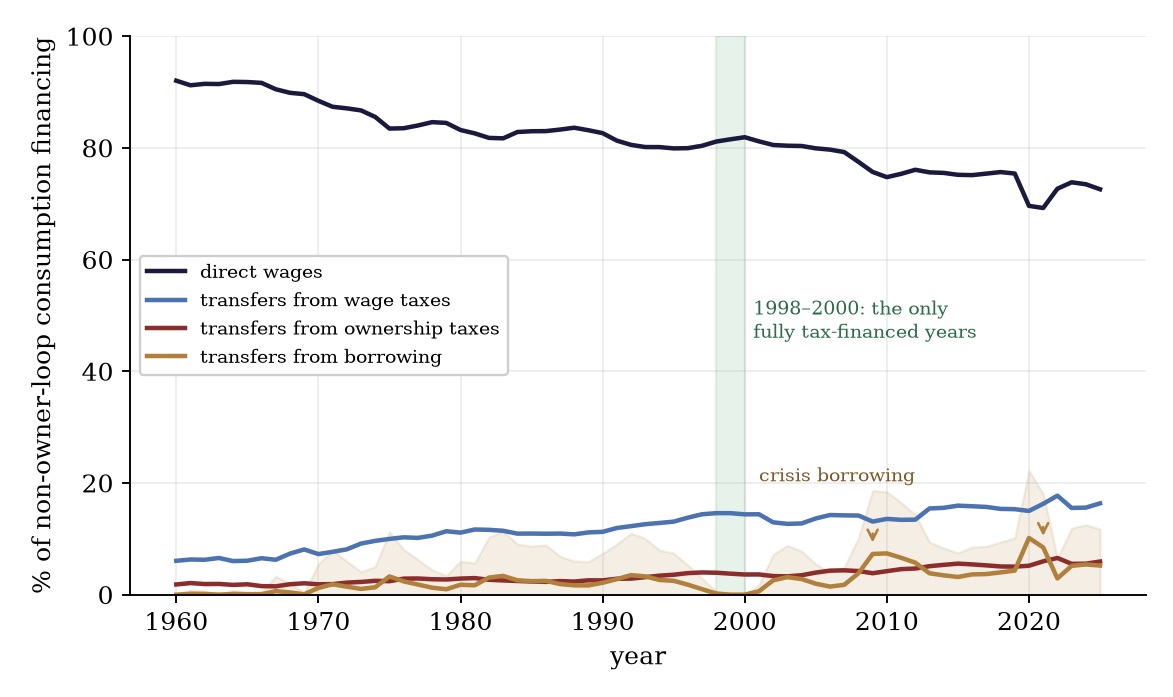
\includegraphics[width=0.88\linewidth]{figures/fig_fourway.png}
\caption{Composition of U.S. consumption financing excluding consumption financed
directly from household capital income, in which owners consume their own
returns, 1962--2025. Lines
are medians across the classification-rule grid; the shaded band spans the
deficit-attribution rules. The direct-wage share fell by about twenty
percentage points over sixty years. Transfers grew while approximately one
quarter of their financing continued to come from taxes on ownership income.
Borrowing financed 19\% of transfers in 2025 and was zero only in
1998--2000. The allocation is pro-rata accounting, not an estimate of tax
incidence.}
\label{fig:fourway}
\end{figure}

\section{Human-required tasks}\label{app:human}

Let Appendix~\ref{app:environment}'s set $H$ have positive measure $|H|$: tasks machines cannot hold --- by capability residue, by verified preference for human hands, or by law --- with $H$-wage $w_H$. Let machines grow unboundedly better at every task outside $H$: $\gamma (x) \to 0$ there, a capability improvement confined to the tasks machines can hold. The interior replacement conditions need not price a worker employed only in $H$. Assume, in a common numeraire, that the rental $c$ remains bounded and the machine work outside $H$ has total unit cost tending to zero. This is a price-path condition: what vanishes is the cost of machine work, $c/\gamma _M(x) = c\cdot \gamma (x)/\gamma _L(x)$. Aghion, Jones, and Jones (2019) raise the strongest stabilizer this paper faces: Baumol concentration --- expenditure concentrating on the sector whose costs refuse to fall (Baumol 1967), here the human-required set --- can preserve labor's share indefinitely. Proposition~\ref{prop:baumol} grants the mechanism its theorem and makes its premise explicit.

\begin{proposition}[Baumol concentration]\label{prop:baumol}
(i) A good with no additional direct requirement for non-produced inputs whose task list contains $H$ has unit cost tending to $|H|\cdot w_H/\gamma _L$ as $\gamma \to 0$ outside $H$: labor's share of its cost tends to one. (ii) Under CES substitution $\sigma _H$ between $H$-content and $H$-light substitutes, the expenditure share of $H$-content tends to 1 if $\sigma _H < 1$, to the taste weight if $\sigma _H = 1$, and to 0 if $\sigma _H > 1$. (iii) On the $\sigma _H < 1$ branch with three categories (machine-made goods, non-produced services, $H$-labor), end-state expenditure splits between the two non-collapsing categories --- non-produced services and $H$-labor --- and labor's aggregate share tends to the $H$-share of that split. A persistent human-required sector can sustain a positive wage--rent ratio.
\end{proposition}

\begin{proof}
(i) $H$-tasks cost $|H|\cdot w_H/\gamma _L$ whatever machines do; each task outside $H$ costs $c\cdot \gamma (x)/\gamma _L(x)$, and the assumed vanishing total cost outside $H$ removes the remainder. (ii) is Appendix~\ref{app:accounting}'s share display with $q$ read as the relative price of $H$-content: the costlier category's share rises with its relative price iff $\sigma _H < 1$, and by (i) that relative price diverges. (iii) A $H$-free good's price vanishes by (i) at $|H| = 0$, so for $\sigma _H < 1$ its share vanishes, leaving the displayed split; setting the $H$ taste weight to zero returns the baseline.
\end{proof}

Two qualifications govern the human-required sector: provenance may be difficult to enforce, and broadcastable demand may concentrate on a small number of performers. \emph{Provenance verification:} preference-based membership binds only if provenance can be verified: suppose buyers carry a taste premium for verified human work, verification catches a false claim with probability $v$, and a caught claim pays a penalty $f$.

\begin{lemma}[the fraud bound]\label{lem:fraud}
A premium on verified human work is sustainable only up to $v\cdot f/(1-v)$: at any higher premium, false claiming is profitable in expectation and entry by fakes competes the premium away. The bound rises in $v$ and in $f$, diverges as $v \to 1$, and collapses to zero as $f \to 0$ for every $v < 1$.
\end{lemma}

\begin{proof}
A false claimant earns the premium with probability $1 - v$ and pays $f$ with probability $v$; expected profit is nonpositive iff the premium is at most $v\cdot f/(1-v)$. The comparative statics and limits are elementary.
\end{proof}

With price-only enforcement $(f \to 0)$ the bound collapses for every $v < 1$: certified-human markets unravel through fakes, not robots. The enforceable core of the human-required set consists of tasks reserved by law and services whose in-person provision makes provenance directly observable. \emph{Superstars:} within $H$, the broadcastable fraction $\psi$ of demand concentrates on top performers (Rosen 1981) while only the in-person remainder is rationed by human capacity.

\begin{lemma}[superstar concentration]\label{lem:superstar}
Let the broadcastable fraction $\psi$ of $H$-expenditure accrue to a set of performers of measure zero, and let the in-person remainder be shared uniformly across the $H$-workforce. The mean $H$-income is unchanged, and the median $H$-income is $(1-\psi )$ times the mean.
\end{lemma}

\begin{proof}
Total $H$-income equals $H$-expenditure whatever its division; the stars carry the fraction $\psi$ on measure zero, every other worker receives the uniform share $(1-\psi )$ times the mean, and a measure-zero top moves no quantile below the top.
\end{proof}

Wherever $H$ employs a minority the economy-wide median worker holds no $H$-task at all, and on the $\sigma _H < 1$ branch the aggregate labor share can persist, even approach one, while the median wage collapses to the participation floor: aggregate rescue, median collapse. The Baumol case also raises the cost of the subsistence bundle: care and teaching put human hours in the subsistence bundle. Extend \ref{app:coverage}'s bundle with $n_s$ hours of $H$-service and coverage becomes $\kappa = qT/(N\cdot (g_s + n_s\cdot w_H/p + q\cdot h_s))$ --- below the $H$-free ratio at every $q$, and further below as the $H$-hour's price rises.

\section{The financing and production accounts}\label{app:effort}

Section~\ref{sec:measurement} quotes two shares; this appendix defines and constructs them. The \emph{labor-origin financing share} asks where the purchasing power used for personal consumption originates. The \emph{full-chain human-effort share} asks how much of the purchaser-price value of consumed production resolves into human labor after intermediates are traced recursively.

For 2004--2023 the financing account uses annual BEA source distributions ranked by equivalized disposable income. Spending beyond current disposable income is kept in an intertemporal bucket rather than assigned to current labor; within current-financed spending, tax incidence and allocation across fungible resources are partially identified and reported as bounds. The labor-origin financing share is 69.6\% [59.8--83.1] in 2004 and 65.8\% [52.7--80.1] in 2023; the model-based 2025 extension is 64.2\% [54.1--81.3].

The production account instead follows the purchaser-price dollar through the production chain. Its BEA benchmark covers 1997--2023: human effort is 50.1\% of consumed production in 1997 and 47.2\% in 2023. Outside that window, a five-specification product-composition model supplies only a model-based extension, at 66.4\% [61.3--68.6] in 1950 and 46.2\% [45.1--47.4] in 2025. Figure~\ref{fig:labor-linkages} marks the benchmark-data windows explicitly.

The long extension suggests that the separation is newer than the postwar starting point, but that inference inherits the weaker status of the outer series.

\textbf{Mapping back to the model.} The production-content account
corresponds to the broader recursion
$\mathbf{c}=\mathbf{A}\mathbf{c}+\boldsymbol{\Lambda}w+\mathbf{B}\mathbf{r}$,
not to the scalar $\lambda$ in the one-sector recipe. Recursive automation
predicts a declining human-effort component as machine-producing and
machine-operating chains shed labor. The financing-origin account supplies
$\varphi_C$ for Appendix~\ref{app:mix}.

\bigskip\par\noindent\rule{0.35\linewidth}{0.4pt}\par\smallskip
\noindent{\footnotesize\singlespacing \textbf{AI use.} This paper was written in collaboration with Claude (Anthropic) and ChatGPT (OpenAI). The theory and its central claims are the authors'; parts of the formalization, proofs, computations, figures, and some initial prose were drafted by Claude Fable 5 and ChatGPT 5.6 Sol under the authors' direction and review. All data were pulled live from public sources; the code and data are public at \url{https://github.com/wilsoniumite/labor}. Errors remain the authors'.\par}

\section*{References}

{\small\singlespacing
\refentry{Acemoglu, D., and D. Autor (2011). ``Skills, Tasks and Technologies: Implications for Employment and Earnings.'' In \emph{Handbook of Labor Economics}, vol. 4B. Elsevier.}
\refentry{Acemoglu, D., and P. Restrepo (2018). ``The Race between Man and Machine: Implications of Technology for Growth, Factor Shares, and Employment.'' \emph{American Economic Review} 108(6): 1488--1542.}
\refentry{Acemoglu, D., and P. Restrepo (2022). ``Tasks, Automation, and the Rise in U.S. Wage Inequality.'' \emph{Econometrica} 90(5).}
\refentry{Acemoglu, D., and P. Restrepo (2026). ``Automation and Rent Dissipation: Implications for Wages, Inequality, and Productivity.'' \emph{The Quarterly Journal of Economics} 141(2): 1521--1579.}
\refentry{Aghion, P., B. F. Jones, and C. I. Jones (2019). ``Artificial Intelligence and Economic Growth.'' In A. Agrawal, J. Gans, and A. Goldfarb (eds.), \emph{The Economics of Artificial Intelligence}, University of Chicago Press.}
\refentry{Allen, R. C. (2001). ``The Great Divergence in European Wages and Prices from the Middle Ages to the First World War.'' \emph{Explorations in Economic History} 38(4): 411--447.}
\refentry{Arnott, R. J., and J. E. Stiglitz (1979). ``Aggregate Land Rents, Expenditure on Public Goods, and Optimal City Size.'' \emph{The Quarterly Journal of Economics} 93(4): 471--500.}
\refentry{Arrow, K. J. (1951). ``An Extension of the Basic Theorems of Classical Welfare Economics.'' In \emph{Proceedings of the Second Berkeley Symposium on Mathematical Statistics and Probability}, University of California Press.}
\refentry{Autor, D. (2015). ``Why Are There Still So Many Jobs? The History and Future of Workplace Automation.'' \emph{Journal of Economic Perspectives} 29(3).}
\refentry{Autor, D., and D. Dorn (2013). ``The Growth of Low-Skill Service Jobs and the Polarization of the US Labor Market.'' \emph{American Economic Review} 103(5): 1553--1597.}
\refentry{Autor, D., F. Levy, and R. J. Murnane (2003). ``The Skill Content of Recent Technological Change: An Empirical Exploration.'' \emph{The Quarterly Journal of Economics} 118(4): 1279--1333.}
\refentry{Baumol, W. J. (1967). ``Macroeconomics of Unbalanced Growth: The Anatomy of Urban Crisis.'' \emph{American Economic Review} 57(3): 415--426.}
\refentry{Bouscasse, P., E. Nakamura, and J. Steinsson (2025). ``When Did Growth Begin? New Estimates of Productivity Growth in England from 1250 to 1870.'' \emph{The Quarterly Journal of Economics} 140(2): 835--888.}
\refentry{Card, D., A. R. Cardoso, J. Heining, and P. Kline (2018). ``Firms and Labor Market Inequality: Evidence and Some Theory.'' \emph{Journal of Labor Economics} 36(S1).}
\refentry{Caselli, F., and A. Manning (2019). ``Robot Arithmetic: New Technology and Wages.'' \emph{American Economic Review: Insights} 1(1).}
\refentry{Clark, G. (2005). ``The Condition of the Working Class in England, 1209--2004.'' \emph{Journal of Political Economy} 113(6): 1307--1340.}
\refentry{Crafts, N. (2022). ``Slow Real Wage Growth during the Industrial Revolution: Productivity Paradox or Pro-Rich Growth?'' \emph{Oxford Economic Papers} 74(1): 1--13.}
\refentry{Diamond, P. A. (1982). ``Aggregate Demand Management in Search Equilibrium.'' \emph{Journal of Political Economy} 90(5).}
\refentry{Diamond, P., and J. Mirrlees (1971). ``Optimal Taxation and Public Production I: Production Efficiency.'' \emph{American Economic Review} 61(1).}
\refentry{George, H. (1879). \emph{Progress and Poverty.}}
\refentry{Grossman, G. M., and E. Rossi-Hansberg (2008). ``Trading Tasks: A Simple Theory of Offshoring.'' \emph{American Economic Review} 98(5).}
\refentry{Gruber, J. (1997). ``The Incidence of Payroll Taxation: Evidence from Chile.'' \emph{Journal of Labor Economics} 15(3, Part 2): S72--S101.}
\refentry{Hagedorn, M., and I. Manovskii (2008). ``The Cyclical Behavior of Equilibrium Unemployment and Vacancies Revisited.'' \emph{American Economic Review} 98(4): 1692--1706.}
\refentry{Hall, R. E. (2005). ``Employment Fluctuations with Equilibrium Wage Stickiness.'' \emph{American Economic Review} 95(1).}
\refentry{Hémous, D., and M. Olsen (2022). ``The Rise of the Machines: Automation, Horizontal Innovation, and Income Inequality.'' \emph{American Economic Journal: Macroeconomics} 14(1).}
\refentry{Hoynes, H., and J. Rothstein (2019). ``Universal Basic Income in the United States and Advanced Countries.'' \emph{Annual Review of Economics} 11.}
\refentry{Jones, D., and I. Marinescu (2022). ``The Labor Market Impacts of Universal and Permanent Cash Transfers: Evidence from the Alaska Permanent Fund.'' \emph{American Economic Journal: Economic Policy} 14(2): 315--340.}
\refentry{Karabarbounis, L., and B. Neiman (2014). ``The Global Decline of the Labor Share.'' \emph{The Quarterly Journal of Economics} 129(1).}
\refentry{Knoll, K., M. Schularick, and T. Steger (2017). ``No Price Like Home: Global House Prices, 1870--2012.'' \emph{American Economic Review} 107(2).}
\refentry{Korinek, A., and J. E. Stiglitz (2019). ``Artificial Intelligence and Its Implications for Income Distribution and Unemployment.'' In A. Agrawal, J. Gans, and A. Goldfarb (eds.), \emph{The Economics of Artificial Intelligence}, University of Chicago Press.}
\refentry{Korinek, A., and D. Suh (2024). ``Scenarios for the Transition to AGI.'' NBER Working Paper 32255.}
\refentry{Kugler, A., and M. Kugler (2009). ``Labor Market Effects of Payroll Taxes in Developing Countries: Evidence from Colombia.'' \emph{Economic Development and Cultural Change} 57(2): 335--358.}
\refentry{Leontief, W. W. (1936). ``Quantitative Input and Output Relations in the Economic Systems of the United States.'' \emph{The Review of Economics and Statistics} 18(3): 105--125.}
\refentry{Lewis, W. A. (1954). ``Economic Development with Unlimited Supplies of Labour.'' \emph{The Manchester School} 22(2): 139--191.}
\refentry{Ljungqvist, L., and T. J. Sargent (2017). ``The Fundamental Surplus.'' \emph{American Economic Review} 107(9): 2630--2665.}
\refentry{Malthus, T. R. (1798). \emph{An Essay on the Principle of Population.}}
\refentry{Manning, A. (2003). \emph{Monopsony in Motion: Imperfect Competition in Labor Markets.} Princeton University Press.}
\refentry{Mas, A., and A. Pallais (2019). ``Labor Supply and the Value of Non-Work Time: Experimental Estimates from the Field.'' \emph{American Economic Review: Insights} 1(1): 111--126.}
\refentry{Moll, B., L. Rachel, and P. Restrepo (2022). ``Uneven Growth: Automation's Impact on Income and Wealth Inequality.'' \emph{Econometrica} 90(6).}
\refentry{Mortensen, D. T., and C. A. Pissarides (1994). ``Job Creation and Job Destruction in the Theory of Unemployment.'' \emph{The Review of Economic Studies} 61(3): 397--415.}
\refentry{Piketty, T., and G. Zucman (2014). ``Capital is Back: Wealth-Income Ratios in Rich Countries 1700--2010.'' \emph{The Quarterly Journal of Economics} 129(3).}
\refentry{Pissarides, C. A. (2000). \emph{Equilibrium Unemployment Theory.} 2nd ed., MIT Press.}
\refentry{Polanyi, K. (1944). \emph{The Great Transformation.}}
\refentry{Ricardo, D. (1817). \emph{On the Principles of Political Economy and Taxation.} Third edition, 1821, adds the chapter ``On Machinery.''}
\refentry{Rognlie, M. (2015). ``Deciphering the Fall and Rise in the Net Capital Share.'' \emph{Brookings Papers on Economic Activity.}}
\refentry{Romer, P. M. (1990). ``Endogenous Technological Change.'' \emph{Journal of Political Economy} 98(5): S71--S102.}
\refentry{Rosen, S. (1981). ``The Economics of Superstars.'' \emph{American Economic Review} 71(5).}
\refentry{Sachs, J. D., and L. J. Kotlikoff (2012). ``Smart Machines and Long-Term Misery.'' NBER Working Paper 18629.}
\refentry{Saez, E., B. Schoefer, and D. Seim (2019). ``Payroll Taxes, Firm Behavior, and Rent Sharing: Evidence from a Young Workers' Tax Cut in Sweden.'' \emph{American Economic Review} 109(5): 1717--1763.}
\refentry{Samuelson, P. A. (1966). ``A Summing Up.'' \emph{The Quarterly Journal of Economics} 80(4).}
\refentry{Shapiro, C., and J. E. Stiglitz (1984). ``Equilibrium Unemployment as a Worker Discipline Device.'' \emph{American Economic Review} 74(3): 433--444.}
\refentry{Shimer, R. (2005). ``The Cyclical Behavior of Equilibrium Unemployment and Vacancies.'' \emph{American Economic Review} 95(1): 25--49.}
\refentry{Sraffa, P. (1960). \emph{Production of Commodities by Means of Commodities.} Cambridge University Press.}
\refentry{Susskind, D. (2017). ``A Model of Technological Unemployment.'' Oxford Department of Economics Discussion Paper 819.}
\refentry{Uzawa, H. (1961). ``Neutral Inventions and the Stability of Growth Equilibrium.'' \emph{The Review of Economic Studies} 28(2): 117--124.}
\refentry{Zeira, J. (1998). ``Workers, Machines, and Economic Growth.'' \emph{The Quarterly Journal of Economics} 113(4).}
}

\bigskip\par\noindent\rule{0.35\linewidth}{0.4pt}\par\smallskip
\noindent{\footnotesize\singlespacing \textbf{Data and computation.} All U.S. figures are gross annual flows computed from BEA national accounts (annual NIPA series retrieved via FRED, 2026 vintage), with Federal Reserve Z.1 balance-sheet lines, BEA fixed-assets stocks, and the CPI for the coverage ratio, and HUD FY2025 fair-market rents for the ceiling grid. Financing splits 1962--2025, coverage ratio 1953--2025, deflator fork 1964--2024 on complete calendar years, with the food comparison from the CPI food index (FRED CPIUFDNS) over the same window. Reported values are medians with min--max bands across a rule grid. Flows are gross. The financing series uses annual BEA source profiles ranked by equivalized disposable income in 2004--2023 with partial-identification bounds and weaker outer extensions. The production series uses the BEA WP2026-01 full-chain benchmark in 1997--2023 and a five-specification NIPA product-composition extension outside that window. \textbf{Notation.} The machine-recipe labor coefficient $\lambda$ is unrelated to the wage-linkage shares $\varphi _C, \varphi _G$ of Appendix~\ref{app:fiscal} and to Acemoglu--Restrepo's task-substitution elasticity $\lambda$; the human-required set $H$ is unrelated to the housing subscript of $T_H$; and the outside option is denoted $s$; the common search-theory symbol $b$ is reserved here for the terminal-input coefficient.\par \textbf{Numerical checks.} The accompanying \texttt{check\_interior.py} checks the replacement derivatives, exact interior category prices, general price bounds, and factor-income cancellation with heterogeneous task assignments. It solves Appendix~\ref{app:equilibrium}'s equilibrium and compares output against an independently specified linear production program with 2,048 task cells. These numerical checks accompany the analytical proofs in the text.\par}

\end{document}
